\documentclass[12pt]{thesis}

% The LaTeX default font is Computer Modern Roman for text and
% math. We will switch to times roman, because that is preferred by
% the Graduate school.  However, you can comment the times fonts and
% uncomment one (or more) of the others to choose a different font set.
\usepackage{mathptmx}   % Times New Roman with matching math fonts
% \usepackage{newcent}  % new century schoolbook font
% \usepackage{bookman}  % bookman font
% \usepackage{fourier}  % Utopia (text) and Fourier (math) font


\usepackage{amsmath}
\usepackage{graphicx}
\usepackage{rotating}
\usepackage{makeidx}
\usepackage{subfig}
\usepackage{indentfirst}
\usepackage{xcolor}

\DeclareMathOperator*{\argmax}{arg\,max}

%% Uncomment the following two lines and comment out the third one
%% if you want to use the Chicago Manual based bibliography.
% \usepackage{thesiscitations}
% \bibliographystyle{thesis}
\bibliographystyle{ieeetr}

%% Change ieeetr in the previous line to any bibliography style you
%% like

%% Uncomment next line if you want chapter titles centered (not
%% approved by SDSMT graduate school)
% \centertitles

%% Uncomment next line to print a double-spaced draft version
% \dsdraft

%% Uncomment next line to print a single-spaced draft version
% \ssdraft

%% Uncomment next line if you are using makeindex to create an index
% \makeindex

%\begin{comment}
%\doctype{thesis}
%\title{A Compative Study of Gnus and Gnats: The Most Important Paper Ever Written}
%\author{Harvey Finklebaum}
%\degree{Doctor of Philosophy in Zoology}
%\defensedate{April 4, 2013}
%\gradyear{2013}
%\department{Zoology}
%\end{comment}

\doctype{thesis}
\title{Temporal PIG: Improving PIG to Resist the Noisy-TV Problem}
\author{David Mathews}
\degree{Masters in Computer Science and Engineering}
\defensedate{TBD}
\gradyear{2024}
\department{Electrical Engineering and Computer Science}

% The following commands add a signature line for each person who needs
% to sign the thesis/dissertation
%\begin{comment}
%\signatureline{Major Professor --- Dimm Whitt, Ph.D., Department of
%  Zoology}
%
%\signatureline{Graduate Division Representative --- E.\ Nigma, Ph.D.,
%  Department of Philosophy}
%
%\signatureline{Committee Member --- Chip Munk, Ph.D., Department of
%  Zoology}
%
%\signatureline{Committee Member --- Gail Force, Ph.D., Department of
%  Meteorology }
%
%\signatureline{Head of the Zoology Department --- Earl E. Byrd, Ph.D.}
%
%\signatureline{Dean of Graduate Education --- Raney Daze}
%\end{comment}

\signatureline{Major Professor --- Larry D. Pyeatt, Ph.D., Department of
	Electrical Engineering and Computer Science}

\signatureline{Graduate Division Representative --- Roger W Johnson, Ph.D.,
	Department of Mathematics}

\signatureline{Committee Member --- Christer Karlsson, Ph.D., Department of
	Electrical Engineering and Computer Science}

\signatureline{Head of the Electrical Engineering and Computer Science Department --- Jeffrey S. McGough, Ph.D.}

\signatureline{Dean of Graduate Education --- Maribeth Price}

\begin{document}

\maketitle

%% Comment the next line to remove the copyright notice.  Read the
%% section on copyright in the Thesis and Dissertation Writing
%% Instructions.
\makecopyright % copyright must go BEFORE \preliminaries

\preliminaries

\begin{abstract}
I present an improvement to the standard PIG algorithm to make it less prone to the Noisy-TV problem. This improvement uses temporal difference learning over the information gain to avoid distraction and promote learning.
\end{abstract}

%% Uncomment the following if you want acknowledgements
\begin{acknowledgments}
  I would like to thank my advisor, Dr.\ Larry D.\ Pyeatt, for all of the support and advice he has given me. Without his aid, this thesis would not be here today. I would also like to thank my brother Jonathan Mathews, for listening to my struggles and telling me how to make all my graphs better.
\end{acknowledgments}


%\begin{comment}
%\tableofcontents
%
%\listoftables
%
%\listoffigures
%\end{comment}


%% Uncomment following lines if you want a list of symbols
%% \gltitle{List of Symbols}
%% \begin{genericlist}
%% \begin{tabular}{ll}
%%   $\mathcal{G}_t$ & Gnat\\
%%   $\mathcal{G}_u$ & Gnu
%% \end{tabular}
%% \end{genericlist}

%% Uncomment following lines if you want a list of keywords
%% \gltitle{List of Keywords}
%% \begin{genericlist}
%% \noindent Gnat, Gnu
%% \end{genericlist}

%% Uncomment following lines if you want a dedication
% \begin{dedication}
% In loving memory of 
% my grandmother.
% \end{dedication}

%% Uncomment following lines if you want a preface
% \begin{preface}
% Before we begin, just let me say one thing.
% Gnat and gnu are both begin with ``gn,'' and
% the purpose of this work was to see if there
% are any other resemblances.
% This thesis has taken 45 years of work, and
% I don't have much time left in this world, but it
% has been worth it.  When the time comes,
% I would like to die as my grandmother did, peacefully in
% her sleep, not screaming like the passengers in her car.
% \end{preface}


\body


\chapter{Introduction}
\begin{figure}
	\begin{center}
		\scalebox{0.5}{\input{images/RL1.pdf_t}}
	\end{center}
	\caption{Reinforcement learning agent and environment.}
	\label{fig:RLagent}
\end{figure}
\section{Reinforcement Learning}
Reinforcement learning (RL) is a subset of Machine Learning where an agent takes actions within an environment to maximize some environmental reward. \cite{Sutton1998} This is a wide field that includes robotic arm manipulation, video game playing, path-planning, and many other areas.

In RL, the environment is the problem space. In the case of an assembly line, the environment would contain the robot arm, the conveyor belt, the items on the belt, and other related aspects. Every time-step, the environment updates. Items move along the belt, the robot arm shifts, etc.

The agent is the part of the program that learns and adapts to its environment. In the same case of the assembly line, the agent is the robotic arm. Every time-step, the agent receives its current state $s$ from the environment. In our current example, the state can be represented as the angle and rotation of the joints in the arm as well as whether the arm’s gripper is open or closed. Once the agent has received its current state from the environment, it decides what action $a$ to take from the set of all possible actions $A$. In our example, this could be telling the arm’s third motor to move to a specific angle and rotation or activating/releasing the gripper.

When an agent takes an action, it gets feedback from the environment in the form of a reward. This reward is a measure of how good the agent’s choice was. For example, if the robot arm successfully created a product, it could get a reward based on the product’s quality. On the other hand, if the robot arm had smashed into a wall, the agent could get a negative reward known as a punishment. The agent can use these rewards to adjust its behavior to maximize the total reward it can get. An example diagram of a reinforcement learning system is shown in \figurename~\ref{fig:RLagent} 

Taken together, the system works as follows. The environment gives a state $s$ to the agent, who uses that state to determine the action $a$ it takes. The environment then gives a reward $r$ to the agent (usually with the next state $s’$) which it uses to learn whether it should take that action again next time it is in that state.

By repeating this process over many time-steps, the agent will eventually learn the best actions to take in order to maximize the total reward.

\subsection{Temporal difference learning}
Temporal difference learning is a common method of reinforcement learning. In temporal difference learning, the agent uses the reward $r$ found to update the value of previous states it has traveled through. The number of previous states that are updated is the value of $N$ in $N$-step temporal difference learning. The value of $N$ is assumed to be $1$ for this study. Temporal difference learning can be done through either value iteration or Q-learning. \cite{Sutton1998}\cite{Ladosz_2022}
\subsubsection{Value Iteration}
In value iteration, the agent internally stores the value of every state $s$ it has visited. These values are stored in a value function $V(s)$ Whenever the agent takes an action $a$, it uses the reward from taking that action $r$ and the value of the new state $V(s')$ to update the value of $s$ according to the following function:

\begin{equation}
V(s) \leftarrow V(s) + \alpha [r + \gamma V(s') + V(s)]
\label{TDLVF}
\end{equation}
Where $V(s)$ is the agent's stored value of state $s$, $r$ is the reward for transitioning from $s$ to $s'$, $\alpha$ is the learning rate, and $\gamma$ is the discount factor.\cite{Sutton1998}

The learning rate $\alpha$ determines how quickly change can happen to $V(s)$. In other words, how quickly the agent can update its internal model when it gets new data. The learning rate is bounded from $(0,1]$. Large values of $\alpha$ (close to 1) cause the agent to rapidly adjust to changes as it finds them. However, this also makes it hard for the agent to hone in on the optimal solution, as it is too easy to over correct. Low values of $\alpha$ on the other hand, take a long time to learn, but approach optimal solutions much more closely in the end. Commonly, reinforcement learning algorithms will reduce the learning rate over time so the agent learns quickly to begin with and then slows down as it approaches its target. This can be done by using the speed of learning (The portion of \ref{TDLVF} inside the square brackets) to calculate $\alpha$. As the agent's value of $V(s)$ approaches the true value of $V(s)$, $\alpha$ will decrease, causing the agent to more slowly approach the true value and avoid jumping over it.

The discount factor $\gamma$ determines what portion of the next state's value $V(s')$ is used to update the current state's value $V(s)$. In other words, $\gamma$ represents how much the agent values future states' reward compared to the immediate reward $r$. The discount factor $\gamma$ is bounded from $(0,1]$. Large values of $\gamma$ (close to 1) cause the agent to value future rewards more. This makes the agent more likely to ignore short-term gains in exchange for long-term payout. On the other hand, small values for $\gamma$ cause the agent to disregard the value of future states, focusing instead on immediate short-term gains.
\subsubsection{Q-learning}
Instead of assigning a value to every state $V(s)$, the agent can assign a value to every state-action pair $Q(s,a)$. Each of these is called a Q-value. In Q-learning, the agent uses Q-values to learn its environment instead of state-based values. Using Q-values instead of value iteration makes some of the math and implementation much easier. This is especially true in stochastic environments.

Stochastic environments have multiple possible resulting states for a single state-action pair. For example, if a robot attempts to open a door there might be a 40\% chance that the robot fails to open the door, a 40\% chance that the door opens successfully, and a 20\% chance that the robot falls over and hurts itself. If the agent was using a value function $V(s)$ it would have to take all three of those resulting end states, their rewards, and the chance of them occurring into account when trying to determine how valuable the current state is. What's worse, that was only one action that could be taken from the current state!

Using Q-values instead means that the value is on the portions of the environment that the agent can control. Every action $a$ is a potential choice the agent could take. $Q(s,a)$ is a direct representation of how valuable a given action $a$ is when in a known state $s$. Q-learning shifts the focus of the agent from the situations it could end up in to the choices it could make in a given situation. In the example above, Q-learning would still take into account the stochastic transitions and different rewards, but that is stored in the value of the action, not the value of the current state.

When using Q-learning, the temporal difference equation becomes as follows:
\begin{equation}
	Q(s,a) \leftarrow Q(s,a) + \alpha [r + \gamma *  \argmax_{a'} Q(s',a') + Q(s,a)]
	\label{eq:TDQVF}
\end{equation}
Where $Q(s,a)$ is the Q-value of the best action in the current state $s$ and $Q(s',a')$ is the Q-value of the best action to be taken from the new state $s'$. $r$ is the reward for transitioning from $s$ to $s'$, $\alpha$ is the learning rate and $\gamma$ is the discount factor.\cite{Ladosz_2022}

\subsection{Intrinsic reward systems}
Although the above explanation of reinforcement learning works in many cases, it struggles to solve problems where environmental rewards are infrequent or spread sparsely throughout the environment. \cite{DBLP:journals/corr/abs-1908-06976}
\cite{FToCFaIM:Jurgen}
One simple example of this is the case of a robot stuck in a maze. Since the robot only gets rewarded when it successfully exits the maze, the robot has no feedback until it succeeds for the first time. For any maze of significantly large size, it is practically impossible for the robot to randomly stumble upon the correct solution. As such, a robot depending on external (environmental) reward to learn is not sufficient to solve this problem.

Intrinsic rewards are one method to allow agents to learn without the presence of environmental rewards. By letting the agent reward itself when it learns about the environment, the agent can learn to maximize its exploration of its environment. Once the agent has explored their environment sufficiently, they can switch to a different algorithm to take advantage of their knowledge. \cite{Rein:VIME}

One simplistic intrinsic reward system is to reward the agent whenever it finds a state it has never encountered before.  \cite{DBLP:journals/corr/TangHFSCDSTA16} This encourages the agent to seek out new states, allowing it to explore its environment more efficiently. This method has problems as discussed later but is significantly better than random exploration. (Taking random actions)

\section{Noisy TV Problem}
The Noisy TV Problem is a particularly difficult scenario when using intrinsic reward systems in reinforcement learning. \cite{DBLP:journals/corr/abs-2008-04388} The problem is as follows: What if within the environment there was a TV with a remote. Whenever the agent was in front of the TV it could press the remote to switch the TV to a random channel.

Many intrinsic reward systems fall prey to this scenario. For example, the intrinsic reward system above that rewards finding new states would consider the TV to be extremely valuable since all it takes is a single action to find a new state! This is significantly better than exploring around over multiple time-steps to find new areas not seen before. What makes this problem particularly difficult is that the agent cannot tell the difference between moving from state to state around the problem space and pressing the button to flip the channel. Both of these things are taking an action based on a given state. Other intrinsic reward systems such as count-based methods, probabilistic methods, and even memory methods also fall prey to this problem.  \cite{DBLP:journals/corr/abs-1908-06976}

\section{Predicted Information Gain (PIG)}
PIG is an algorithm that uses information theory to maximize exploration of the environment. \cite{10.3389/fncir.2013.00037} PIG functions by predicting how much information about the environment the agent will learn for each action it could take, then taking the action with the most information gain. This means that PIG focuses on creating the best model of the world it can, rather than maximizing the reward obtained from the environment.

\subsection{KL-Divergence}
To determine the amount of information that can be gained from entering a new state, PIG uses the Kullback-Leibler (KL) divergence. The KL-divergence determines the similarity of two probability distributions. In our case, it is the average amount of information that would be lost if we represented one probability distribution with code optimized for the other distribution.

The equation for the KL-divergence is as follows:
\[D_{KL} (\Theta_{as\cdot} || \hat{\Theta}_{as\cdot}) := \sum_{s' = 1}^{ N} \Theta_{ass'} \log_{2}(\frac{\Theta_{ass'}}{\hat{\Theta}_{ass'}})   \]
Where $\Theta$ is the true probabilities of state transition from state $s$ to state $s'$ by taking action $a$, $\hat{\Theta}$ is the agent's estimation of $\Theta$ based on its experiences, and $N$ is the number of valid possible state transitions from $s$ to $s'$.

\subsection{Information Gain/Missing Information}
PIG calculates the amount of information that would be gained when taking a specific action by averaging the amount of information that each state transition would give multiplied by the chance of achieving that state transition. The equation is as follows:

\[ PIG(a,s) := E_{s^{*},\Theta|\vec{d}} [I_{G}(a,s,s^{*})] = \sum_{s*} \hat{\Theta}_{ass^{*}}D_{KL}(\hat{\Theta}_{as\cdot}^{a,s \rightarrow s^{*}} || \hat{\Theta}_{as\cdot}) \]
Where $s^{*}$ is a valid resulting state due to taking action $a$ in state $s$ and $\hat{\Theta}_{as\cdot}^{a,s \rightarrow s^{*}}$ is the updated model of $\hat{\Theta}_{as\cdot}$ if a transition from $s$ to $s^{*}$ was observed.

Intuitively, $D_{KL}(\hat{\Theta}_{as\cdot}^{a,s \rightarrow s^{*}} || \hat{\Theta}_{as\cdot})$ is a measure of how different our new model would be compared to our current model if we successfully transitioned from $s$ to $s^{*}$. The PIG algorithm takes this measure for every state $s^{*}$ it could end up in, then averages them to find out how valuable that action is in total. Pig then uses those values to pick the action $a$ that would teach it the most about its environment.

Since the above equation is fully dependent on our internal model rather than the true model of the environment, it is updated whenever new data is learned and can be applied even when the agent is unaware of the true nature of the environment (As is the case in most real-world problems). In fact, the above equation can even be applied when the agent has no understanding of the problem space whatsoever but merely has a method of observing and interacting with its environment.

\section{Thesis Statement}
The PIG algorithm still falls prey to the Noisy TV problem. When in the Noisy TV state, the PIG algorithm will predict that there is a lot of information to be gained by using the remote. This is because pressing the remote takes the agent to a state significantly different from the state it is currently in, making the KL-divergence between the two states large. Even though the PIG algorithm takes the weighted average of the information gain based on how likely it is to get to that state, it will still consider pressing the remote to be valuable because every state it could reach through the Noisy TV has a high KL-divergence.

The largest cause of this problem is that there is no confirmation that information has actually been learned. The PIG algorithm predicts future information gain based on it’s current data, but it never confirms that its prediction was correct.

As such, I suggest changing the PIG algorithm to make it more robust to the Noisy TV problem. After each time-step, the new algorithm will re-calculate the Predicted Information Gain with the updated models from including the previous step. It will then compare the prediction from before with the new prediction. If information was actually learned the new prediction will be lower then the previous prediction as the total amount of information left to be learned has decreased. This decrease in unlearned information will then be normalized and used as an intrinsic reward. When this new method, Temporal Predicted Information Gain (TPIG), encounters the Noisy TV problem it will quickly realize that although the TV looks like it will provide a large amount of information, it actually provides very little that is useful.

\section{Methods}
%Include methods for testing to determine Thesis statement validity.
To determine the validity of the TPIG method, a grid-world simulation (described below) will be created. The original PIG algorithm, the TPIG algorithm, and a random action baseline will be tested on the simulation and their results compared. $\epsilon$-greedy versions of the PIG and TPIG algorithms will also be tested.

The full project will be available on github.\cite{TPIG:github} This repository will include the simulations used in this paper along with the data gathered and a final copy of this document.

\subsection{Metrics}
The metrics for comparison will be the learning rate (How fast the algorithms approach an optimal solution), the distraction rate (How many times the agent views the Noisy TV), and the internal model accuracy (The KL-divergence between the true model and the agent's model after a given amount of time). These measurements will be taken every time-step and recorded. Their results will then be graphed and compared to each other.


\subsection{Simulation}
The simulation will be a grid-world. The simulation will declare which state the agent will start in. There is no goal state; instead, each episode will run for a given number of time steps before terminating.

In every state the agent will have four actions, one for each direction the agent can travel. Moving into a wall will return the agent to its current state. One of the states will have a Noisy TV that is activated when the agent moves into the TV. Activating the Noisy TV will randomize the Noisy-TV variable in the state space.

Multiple simulations will be used for testing. Each simulation will have a different number of Noisy-TV's. These simulations are shown in figure 
\figurename~\ref{Fig:Sim} and discussed in more depth later in the paper.
\begin{figure}
	\begin{center}
		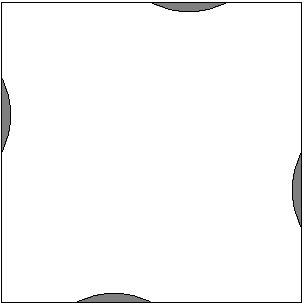
\includegraphics[scale=0.75]{"images/4-TV.pdf"}
		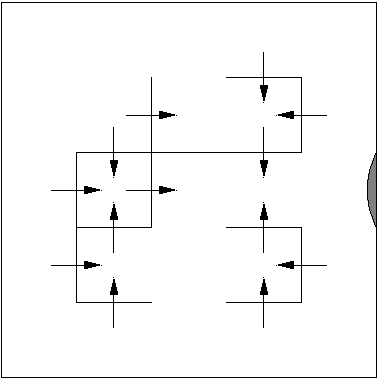
\includegraphics[scale=0.75]{"images/1-TV.pdf"}
		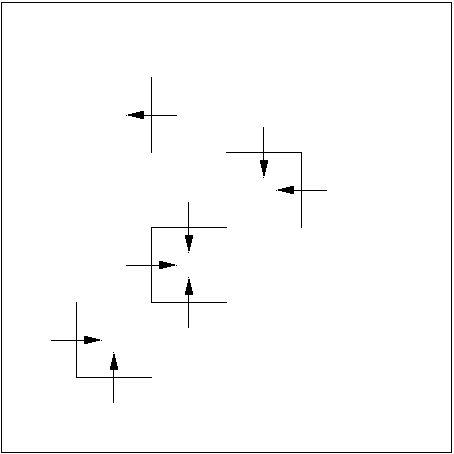
\includegraphics[scale=0.75]{"images/No-TV.pdf"}
	\end{center}
	\caption{Three example simulations. Each semi-circle represents a Noisy-TV}
	\label{Fig:Sim}
\end{figure}
%True model and internal model for KL-divergence comparisons does not take Noisy-TV variable into account. This prevents exploding KL-divergences and represents how the Noisy TV has to effect on state transitions and is just noise.

\chapter{Methods}
\section{Simulation}
The simulations are a grid world. Agents can move in any of the four cardinal directions. If an agent walks into a wall, it does not change states. Every simulation is stored in a file for later access and use.
\subsection{Diagrams}
Three simulations were used to test the agent and its policies. Each policy was tested on all three simulations. These simulations are shown in \figurename~\ref{Fig:Sim}. The first of these is a 4x4 and has multiple Noisy-TV's. The second is a 5x5 with a single Noisy-TV. The final simulation is a 6x6 without any Noisy-TV's. The no-TV simulation serves as a control for how policies act without any distractions.
\subsection{Implementation}
The simulation program is capable of reading in a simulation from a special ``.sim" file. The user can then forcefully change the agent's location or use the built in ``takeAction" function to move the agent according to the transition rules. The user can also print out simulations to a PDF file for easy viewing.

The transition rules are defined inside the simulation class. By default, there is a 90\% chance of taking the desired action and a 10\% chance of staying in the same state instead. Moving into a wall has a 100\% chance of leaving the agent in the same state. Moving into a Noisy-TV is the same as moving into a wall, but the noise variable in the state is incremented, simulating how the Noisy-TV looks different every time the remote is used to flip the channel.

Due to the complications of data storage, the current simulation stores all transitions as a two-dimensional vector that is indexed by a state-action pair. (s,a) pair. This means that noise is not taken into account in the starting state when indexing observed state transitions. This issue is not significant since the only states with noise are the Noisy-TV states and all state comparisons using the Noisy-TV states are done using functions that take the noise into account. In addition, since the noise represents the ``channel" of the Noisy-TV this is an accurate representation as all Noisy-TV states are technically ``In the same room". Future work could detach these states, potentially making this problem harder.

A more technically accurate representation would have each Noisy-TV state transition be stored relative to the noise of the state that the agent moved from. Essentially having each state transition with a noisy state be stored in its own portion of the (s,a) indexed array. However, since the noise has no effect on the actual transitions of the simulation, storing it in this way is impractical and confusing.

\section{Policies}
Policies define how the agent selects an action to take based on its internal model. The variable $\pi$ is used to denote the policy. In mathematical terms: $\pi(a | s)$
\subsection{Implementation}
Every policy has functions to select actions and update their internal model. The policy selects an action $a$ based on its current state $s$. This action $a$ is then passed to the simulation which returns the new state $s'$ that the agent transitions to. This set of $(s,a,s')$ defines a unique state transition.

The policy can use a state transition to update its internal model. When it does so, it adds the state transition to its list of observed transitions. All policies (even those that don't use their internal model for decisions) are capable of updating their internal model.
\subsection{Random Walk}
The Random Walk algorithm always chooses a random action. Each action has an equal probability (25\%) of being chosen. The Random Walk algorithm observes state transitions and updates its internal model as normal, but never uses those observations to affect its decision process. In this paper, the Random Walk algorithm is used as a baseline for algorithm comparisons.

\subsection{Predicted Information Gain (PIG)}
The PIG algorithm calculates the predicted information gain of every action it could take based on its model, then selects the action with the largest potential gain. It does this by using the Kullback-Leibler divergence to estimate how much information remains to be gathered from each $(s,a)$ pair. The action from the $(s,a)$ pair with the highest value is then chosen.

The Kullback-Leibler divergence is defined as follows:
\[D_{KL} (\Theta_{sa\cdot} || \hat{\Theta}_{sa\cdot}) := \sum_{s' = 1}^{ N} \Theta_{sas'} \log_{2}(\frac{\Theta_{sas'}}{\hat{\Theta}_{sas'}})   \]
Where $\Theta_{sa\cdot}$ is the true transition probabilities when starting in state $s$ and taking action $a$ and $\hat{\Theta}_{sa\cdot}$ is the agent's estimated transition probabilities when starting in state $s$ and taking action $a$  based on the transitions they have observed and stored. Similarly, $\Theta_{sas'}$ is the true transition probability of a transition from state $s$ to state $s'$ when taking action $a$ and $\hat{\Theta}_{sas'}$ is the agent's estimated transition probability from state $s$ to state $s'$ when taking action $a$ based on the transitions they have observed and stored.

The Kullback-Leibler divergence is often used in information theory to estimate the information difference from one model to another. In the PIG algorithm, the Kullback-Leibler divergence is used to estimate the potential information that could be gained from taking a specific action.
This is done through the following equation:
\[ PIG(a,s) := \sum_{s*} \hat{\Theta}_{ass^{*}}D_{KL}(\hat{\Theta}_{as\cdot}^{a,s \rightarrow s^{*}} || \hat{\Theta}_{as\cdot}) \]
Where $s^{*}$ is a potential future state that could be transitioned to and $\hat{\Theta}_{as\cdot}^{a,s \rightarrow s^{*}}$ is the observed transition probabilities from state $s$ when taking action $a$ after a transition $(s,a,s^{*})$ has been observed and used to update the internal transition probabilities in the model.

In an ideal scenario, the true transition probabilities $\Theta_{as\cdot}$ would be used instead of $\hat{\Theta}_{as\cdot}^{a,s \rightarrow s^{*}}$ for this calculation. However, since the agent does not have access to the true transition probabilities, $\hat{\Theta}_{as\cdot}^{a,s \rightarrow s^{*}}$ is used as an estimate to allow the agent to learn. There is no oracle in this study, however if an oracle did exist, the true transition probabilities could be used instead to potentially great effect.

Conceptually, the agent's estimate $\hat{\Theta}$ will approach the true distribution $\Theta$ as the agent gathers more data. As the gathered data approaches infinity, the agent's estimate $\hat{\Theta}$ will approach the true distribution $\Theta$. In mathematical terms:

\[ \lim_{d \rightarrow \infty} D_{KL}( \Theta_{as\cdot} || \hat{\Theta}_{as\cdot}) = \lim_{d \rightarrow \infty} \sum_{s' = 1}^{ N} \Theta_{sas'} \log_{2}(\frac{\Theta_{sas'}}{\hat{\Theta}_{sas'}}) = 0\]
This can be clearly seen, as $\frac{\Theta_{sas'}}{\hat{\Theta}_{sas'}}$ approaches 1 as more data is gathered and the $\lim_{x \rightarrow 1} \log_{2}(x)$ is 0.

The Kullback-Leibler divergence and (consequently) PIG algorithm do have some inherent limitations that needed to be handled in physical implementation. In the following sections, these limitations and my methods of resolving them are discussed in depth.

The method above is not the only implementation of the PIG algorithm. There are advanced versions of PIG that predict the information gain for multiple time steps in the future. However, these methods are outside the scope of this paper. Future work could be done on testing these methods to determine their effectiveness.

\subsubsection{Unobserved Transitions}
Due to the nature of the Kullback-Leibler divergence, every state that exists in $\Theta$ but not in $\hat{\Theta}$ will produce a result of $\infty$, as the $\lim_{x \rightarrow 0} \frac{\Theta}{x} = \infty$. This means that the Kullback-Leibler divergence is only valid if $\Theta$ and $\hat{\Theta}$ are one-to-one over their probability distributions. Thankfully, this is not an issue when running the PIG algorithm in practice. Since $\hat{\Theta}_{sas^{*}}$ is 0 when $\hat{\Theta}_{as\cdot}^{a,s \rightarrow s^{*}}$ is transitioning to a new (undiscovered) state $s^{*}$, we can shortcut past the actual calculation whenever  $\hat{\Theta}_{as\cdot}$ and their predicted counterpart $\hat{\Theta}_{as\cdot}^{a,s \rightarrow s^{*}}$ are different sizes (when $s^{*}$ has not been found yet), returning a 0 instead.

This method also applies when the algorithm is just beginning and $\hat{\Theta}_{as\cdot}$ is empty. In this early case, any action is optimal. When gathering data for the algorithm comparisons, $\Theta$ and $\hat{\Theta}$ are not the same size and this problem does become an issue. The specifics of how this is resolved will be discussed in the results section.

\subsubsection{PIG Closed Minded Models}
The Kullback-Leibler divergence returns 0 when the probabilities of its two inputs are the same. However, this provides a problem when the PIG algorithm is learning. Specifically, this prevents the PIG algorithm from exploring new states.

When the PIG algorithm observes a transition for the first time, it stores the probability of that transition $(s,a,s')$ occurring as 100\%. This is regardless of what the true transition probability is. When PIG has explored for a while and comes back to that state $s$, it will predict that the transition $(s,a,s')$ is still 100\% when it takes action $a$ regardless of what the true probability actually is. Since the predicted probability and the measured probability of $(s,a,s')$ are both the same (100\%) the Kullback-Leibler divergence will return 0 and PIG will consider the related action $a$ as being less valuable than other actions.

This makes the PIG algorithm focus on areas it has already explored and found variance in, to the detriment of exploring anywhere it has only touched once. To fix this issue, the PIG algorithm in my implementation initializes the total number of observed transitions to 1 instead of 0. In other words, the number of total transitions the agent has observed is one less than the number of transitions they \b{think} they have observed.

Intuitively, I have tricked the PIG algorithm into thinking it has observed a transition that does not exist. As such, the PIG algorithm will always think that there is more to learn about every state-action pair $(s,a)$ it has ever encountered. As a result, the probabilities of the two inputs of the Kullback-Leibler divergence function will never be the same, and the PIG algorithm will never stop exploring. Although this method does modify the original PIG algorithm, the PIG algorithm will still converge to a Kullback-Leibler divergence of 0. As such, I feel this change is justified.

\subsection{Erratic Predicted Information Gain (EPIG)}
The EPIG algorithm is exactly the same as the PIG algorithm, except that it follows an $\epsilon$-greedy model. This means that whenever EPIG selects an action, it has an $\epsilon$\% chance to select a different action instead. Since EPIG occasionally takes a different action than the ``optimal'' one, it is capable of escaping from infinite loops such as the Noisy-TV. Except for the graphs specifically testing $\epsilon$, in this implementation, $\epsilon$ is set to 10\%.

\subsection{Temporal Predicted Information Gain (TPIG)}
The TPIG algorithm uses the Kullback-Leibler Divergence to calculate how much information is in a given $(s,a)$ pair. After observing a state transition $(s,a,s')$ it calculates the amount of information there is remaining to be learned both before and after the transition is used to update its internal model. TPIG then takes the difference between the two calculations. This difference is used as a reward to determine future actions. The reward function is as follows:
\begin{equation}
	Reward(s,a,s') := D_{KL}(\hat{\Theta}_{a,s \rightarrow s'}^{t-1} || \hat{\Theta}_{as\cdot}^{t-1}) - D_{KL}(\hat{\Theta}_{a,s \rightarrow s'}^{t} || \hat{\Theta}_{as\cdot}^{t})
\label{eq:TPIGReward}
\end{equation}
Where $\hat{\Theta}_{as\cdot}^{t-1}$ is the transition probabilities given before the state transition has been updated and $\hat{\Theta}_{a,s \rightarrow s'}^{t-1}$ is the predicted transition probabilities if the $(s,a,s')$ transition was observed. After the $(s,a,s')$ transition has been used to update the model, $\hat{\Theta}_{as\cdot}^{t}$ is the new transition probabilities after the update. $\hat{\Theta}_{a,s \rightarrow s'}^{t}$ is the predicted transition probabilities if a second transition $(s,a,s')$ was observed.

The reward is then used to update the internal values of the $(s,a)$ pairs. These internal values known as Q-values are used to determine the optimal action to take.
The formula for updating the Q-values is a standard temporal difference equation \eqref{eq:TDQVF}. A simplified form of this equation is shown below:
\[Q_{new} = Q_{old} + \alpha(Reward + \gamma Q_{new} - Q_{old})\]
Where $Q_{old}$ is the Q-value of the best action in the current state $s$ and $Q_{new}$ is the Q-value of the best action to be taken from the new state $s'$. The learning rate $\alpha$ and discount factor $\gamma$ are both set to $0.9$. Q-values were initialized to 1.

To determine which action to take, TPIG checks its internal model of Q-values. The action $a$ that has the highest Q-values for its current state $s$ is chosen. This is formalized in the following equation:

\[ TPIG(s) = \argmax_a  Q(s,a)\]

\subsubsection{TPIG and Infinity}
In the initial exploration for TPIG, the Kullback-Leibler divergence will return $\infty$. This is because there are no known transitions in $\hat{\Theta}_{sa\cdot}$. To prevent these results from breaking the algorithm, any infinities returned by the Kullback-Leibler divergence is replaced with a 0 when the Reward is calculated.

To avoid punishing the model when discovering new states, the reward is set to 0 if it is a negative number. Similarly, any Q-values that are infinity are normalized to 0 before the function to update the Q-values is called.

\subsubsection{Conceptual Explanation}
Whenever TPIG observes a state transition $(s,a,s')$, it uses the Kullback-Leibler divergence to calculate how much information there is left to be gained. It does this calculation both before and after it updates its internal model with the observed transition.

TPIG then compares the amount of information there was before and after its update. If TPIG learned something, the total information left to be learned should be less after the update then before. TPIG uses the value of this decrease to reward itself. The faster TPIG learns from taking an action, the more TPIG values that action.

Simply, TPIG takes the action that it has experienced will make it take the most information from its environment. This is in contrast to PIG which takes the action that it predicts will teach it the most.

\subsection{Erratic Temporal Predicted Information Gain (ETPIG)}
The ETPIG algorithm is exactly the same as the PIG algorithm, except that it follows an $\epsilon$-greedy model. This means that whenever ETPIG selects an action, it has an $\epsilon$\% chance to select a different action instead. Except for the graphs specifically testing $\epsilon$, in this implementation, $\epsilon$ is set to 10\%.

\chapter{Results}
Each of the above policies were tested on all three simulations as shown in \figurename~\ref{Fig:Sim}. Every policy was run 100 times on each simulation. The policies were evaluated on three criteria. Their results were then compared to each other to determine the effectiveness of each policy. The metrics used for this comparison are as follows:
\begin{figure}
	\begin{center}
		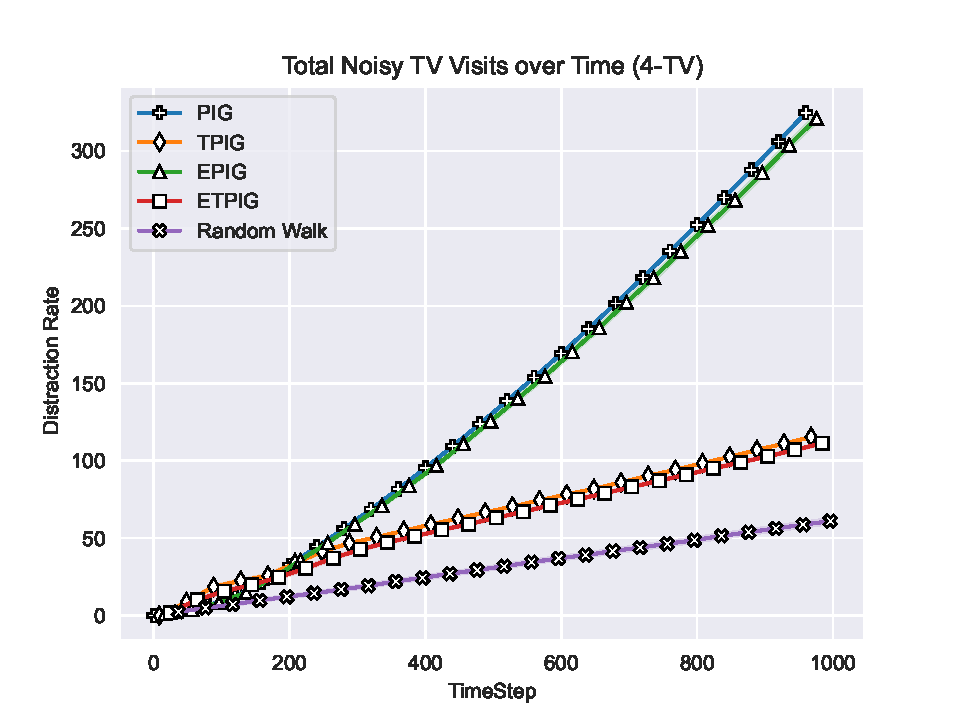
\includegraphics[scale=0.8]{"images/Distraction_Rate_4-TV.pdf"}
	\end{center}
	\caption{Distraction Rate of all Five Policies for 4-TV simulation}
	\label{Fig:DRFP4TV}
\end{figure}
\begin{figure}
	\begin{center}
		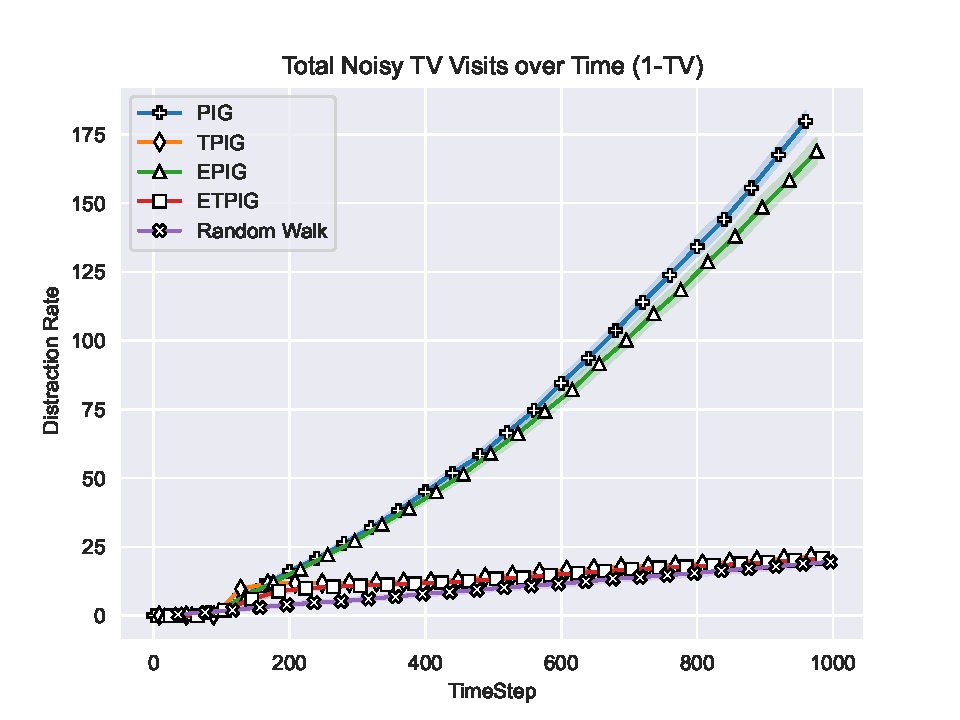
\includegraphics[scale=0.8]{"images/Distraction_Rate_1-TV.pdf"}
	\end{center}
	\caption{Distraction Rate of all Five Policies for 1-TV simulation}
	\label{Fig:DRFP1TV}
\end{figure}
\begin{figure}
	\begin{center}
		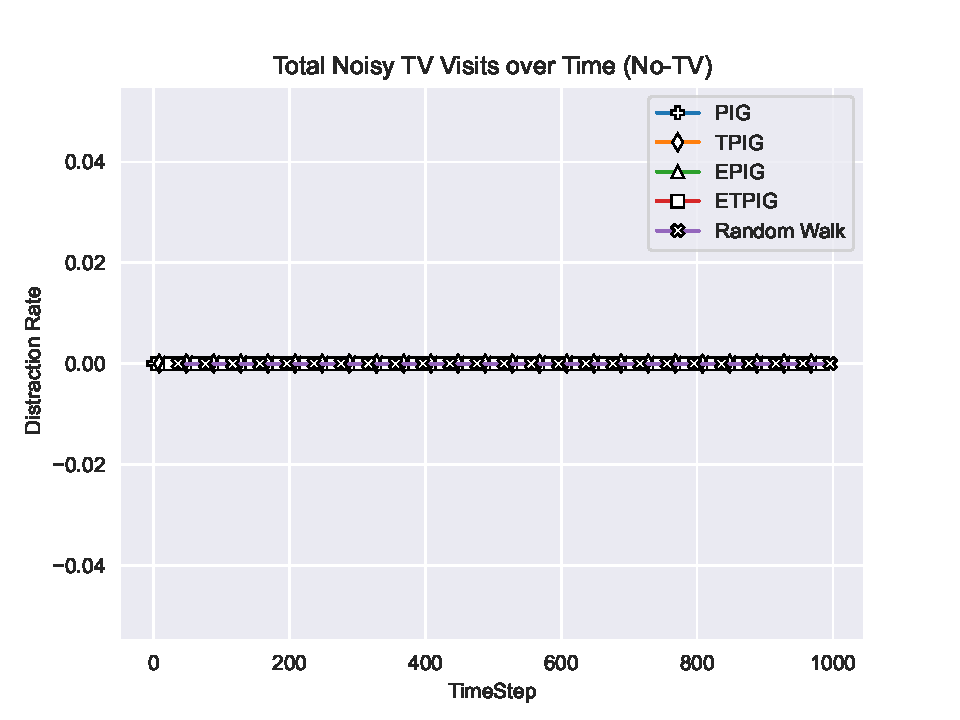
\includegraphics[scale=0.8]{"images/Distraction_Rate_No-TV.pdf"}
	\end{center}
	\caption{Distraction Rate of all Five Policies for No-TV simulation}
	\label{Fig:DRFP0TV}
\end{figure}

\begin{itemize}[]
	\item Distraction Rate: Total number of times algorithm used the Noisy-TV
	\item Learning Rate: Number of unobserved state transitions in the simulation.
	\item Model Accuracy: Accuracy of policy model with respect to the true model.
\end{itemize}

\section{Distraction Rate}
\figurename~\ref{Fig:DRFP4TV}, \ref{Fig:DRFP1TV}, and \ref{Fig:DRFP0TV} are comparisons of the distraction rate of all five policies. Every time the agent activated the Noisy-TV, the distraction rate counter was increased by 1. As such, the fewer times a given algorithm is distracted by the Noisy-TV the better.

In all three simulations, the baseline Random Walk algorithm was distracted the least. In the simulations with Noisy-TV's, the PIG algorithm was distracted heavily by the Noisy-TV. The TPIG algorithm, in comparison, was initially distracted but quickly learned to ignore or avoid the distraction.

In the 1-TV simulation, (\figurename~\ref{Fig:DRFP1TV}) the TPIG algorithm approached Random Walk in how effectively it ignored the Noisy-TV. In the 4-TV simulation, (\figurename~\ref{Fig:DRFP4TV}) however, TPIG does not approach Random Walk's effectiveness, but does perform much better than PIG does. In the simulation without any Noisy-TV's, (\figurename~\ref{Fig:DRFP0TV}) all algorithms performed equally well on this metric, since there were no distractions.


Both PIG and TPIG were improved with the adding of an $\epsilon$-greedy component. This is expected, as adding an $\epsilon$ chance to randomly move allows the algorithm to ``free" itself from distracting loops.


%\begin{sidewaysfigure}
%	\begin{center}
%		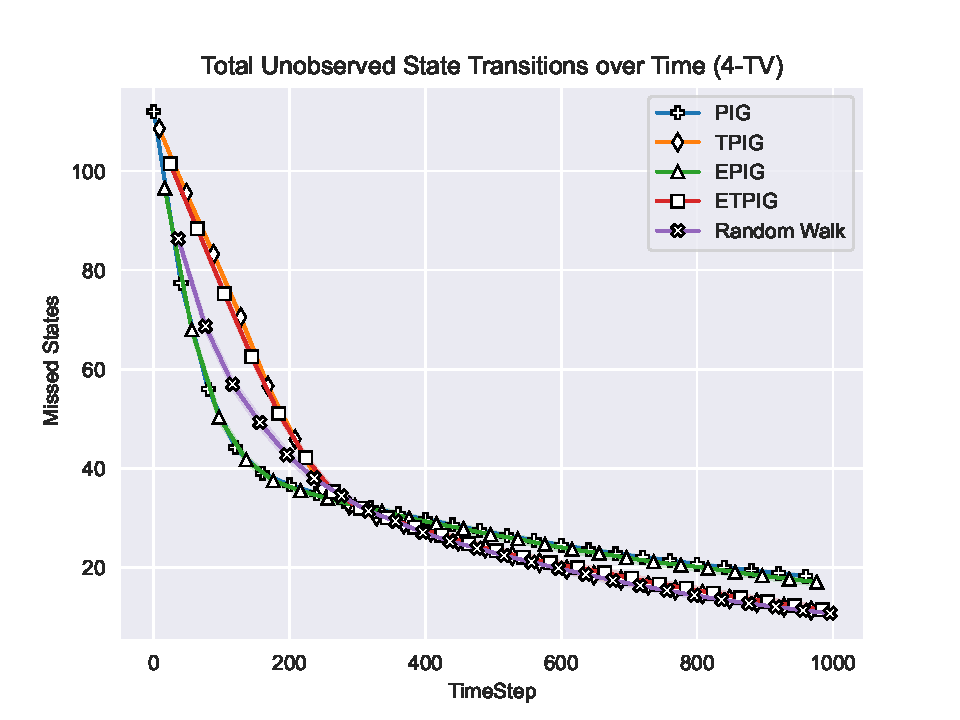
\includegraphics[scale=0.7]{"images/Missed_States_4-TV.pdf"}
%		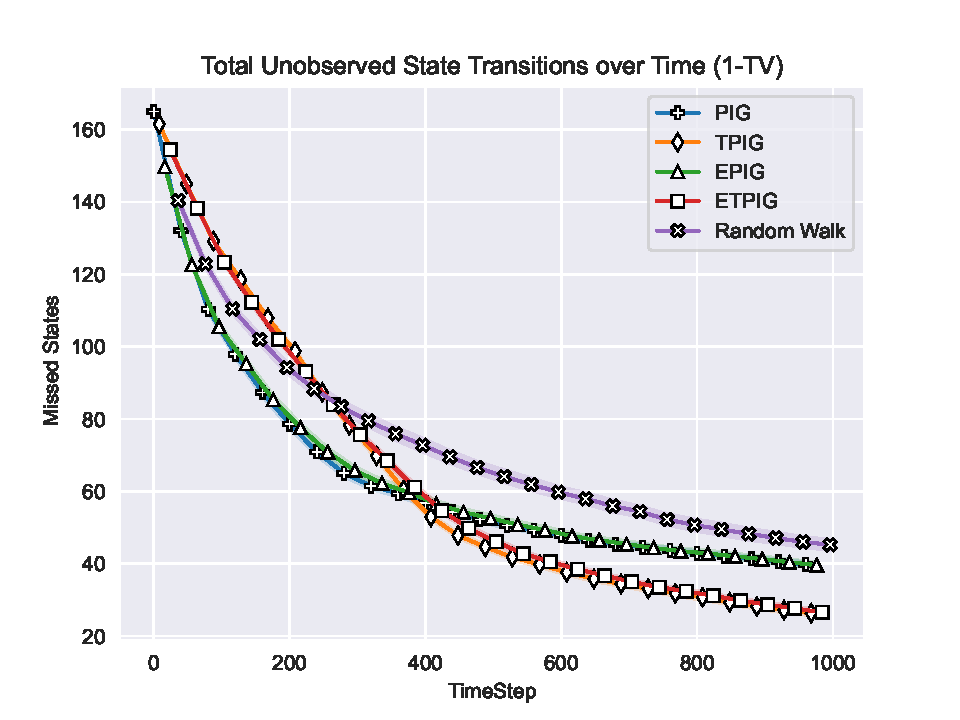
\includegraphics[scale=0.7]{"images/Missed_States_1-TV.pdf"}
%		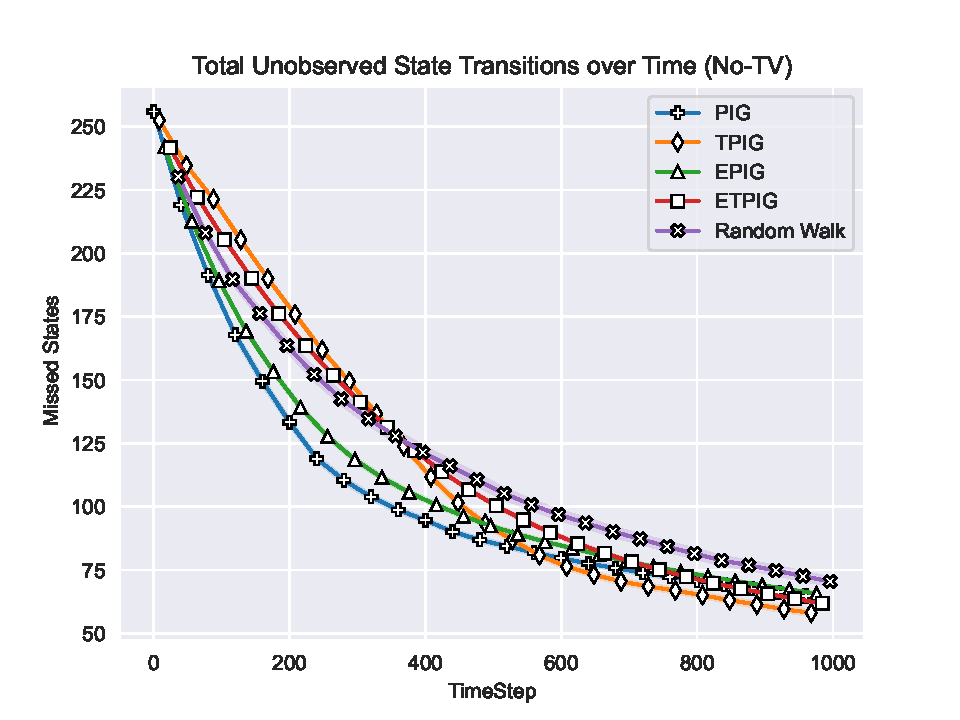
\includegraphics[scale=0.7]{"images/Missed_States_No-TV.pdf"}
%	\end{center}
%	\caption{Missed States of all Five Policies for simulations with Four TV's (Left), No TV (Middle) and One TV(Right)}
%	\label{Fig:MSFP}
%\end{sidewaysfigure}

\section{Learning Rate}
\figurename~\ref{Fig:MSFP4TV}, \ref{Fig:MSFP1TV}, and \ref{Fig:MSFP0TV} are comparisons of the learning rate of all five policies. Each missed state is a state transition that exists in the true model, but has not been found yet by the agent. As such, the faster the number of missed states for the algorithm decreases, the faster it is learning about its environment.

Compared to the Random Walk baseline, the PIG algorithm performed better in the simulations with 1-TV (\figurename~\ref{Fig:MSFP1TV}) or No-TV (\figurename~\ref{Fig:MSFP0TV}). In the 4-TV simulation (\figurename~\ref{Fig:MSFP4TV}), PIG performed better initially, but worse in the end. The TPIG algorithm, in comparison, initially performed worse than both PIG and the Random Walk for all three simulations. After enough time, however, the TPIG algorithm performs better than both Random Walk and PIG in all three simulations.

The $\epsilon$-greedy implementations had no significant impact on the base algorithms. This is interesting behavior, as it demonstrates that the exploration of new transitions was minimally effected by small values of $\epsilon$ (10\%).


\begin{figure}[p]
	\begin{center}
		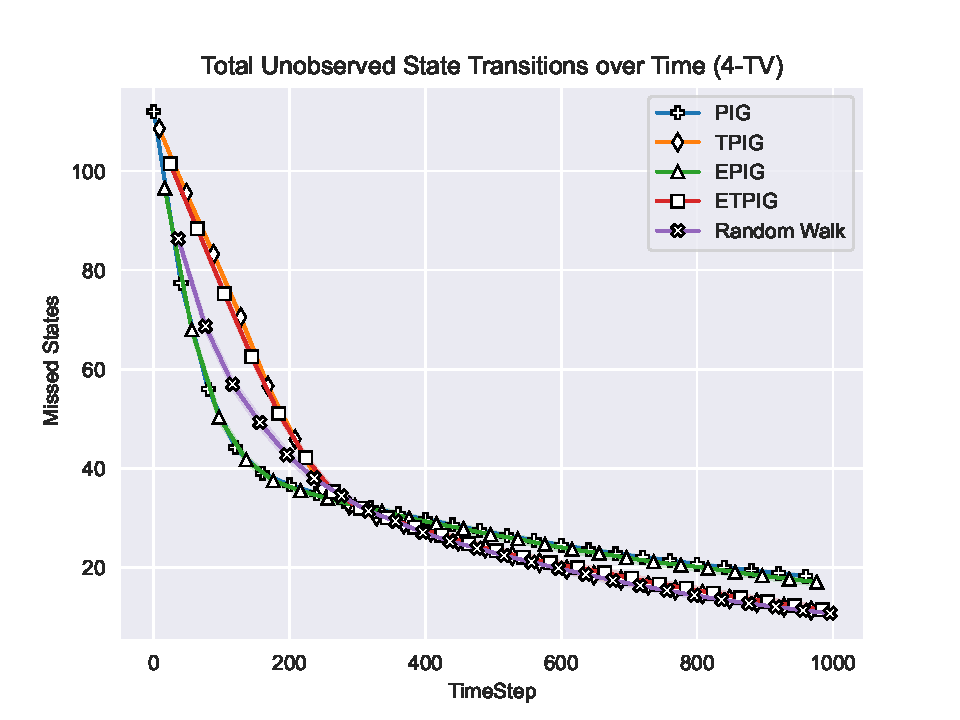
\includegraphics[scale=0.8]{"images/Missed_States_4-TV.pdf"}
	\end{center}
	\caption{Missed States of all Five Policies for 4-TV Simulation}
	\label{Fig:MSFP4TV}
\end{figure}
\begin{figure}
	\begin{center}
		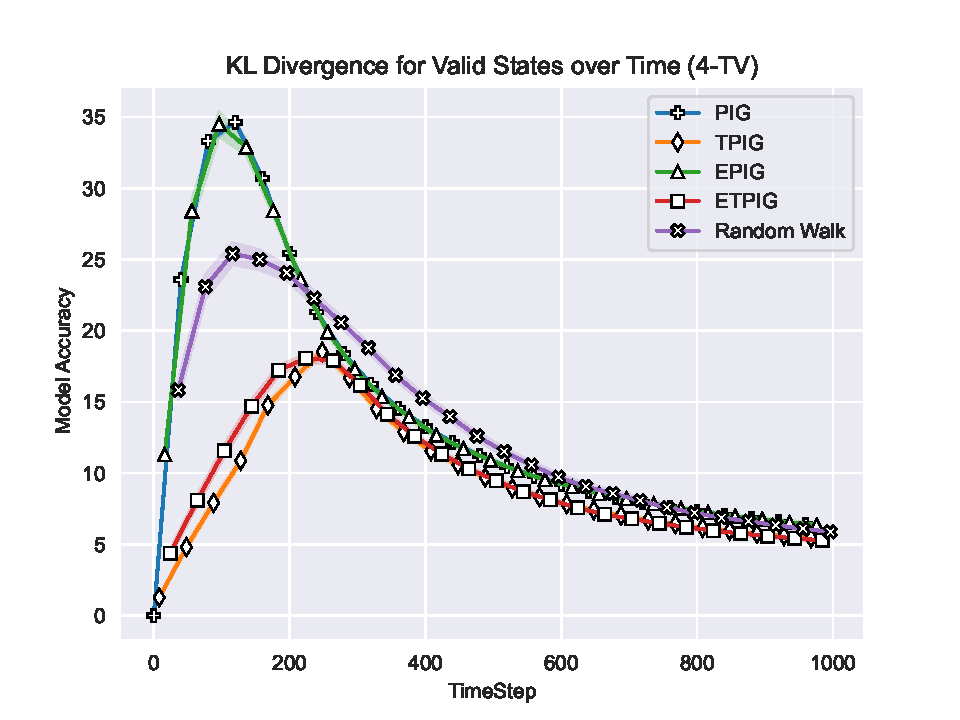
\includegraphics[scale=0.8]{"images/Model_Accuracy_4-TV.pdf"}
	\end{center}
	\caption{Model Accuracy of all Five Policies for 4-TV simulation.}
	\label{Fig:MAFP4TV}
\end{figure}

\begin{figure}[p]
	\begin{center}
		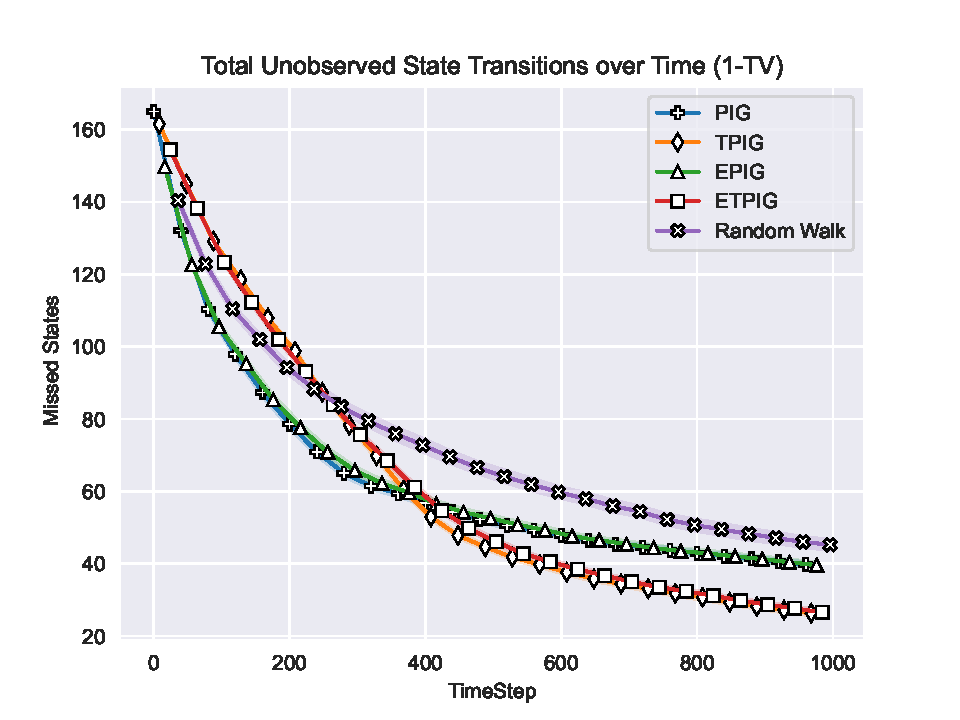
\includegraphics[scale=0.8]{"images/Missed_States_1-TV.pdf"}
	\end{center}
	\caption{Missed States of all Five Policies for 1-TV Simulation}
	\label{Fig:MSFP1TV}
\end{figure}
\begin{figure}
	\begin{center}
		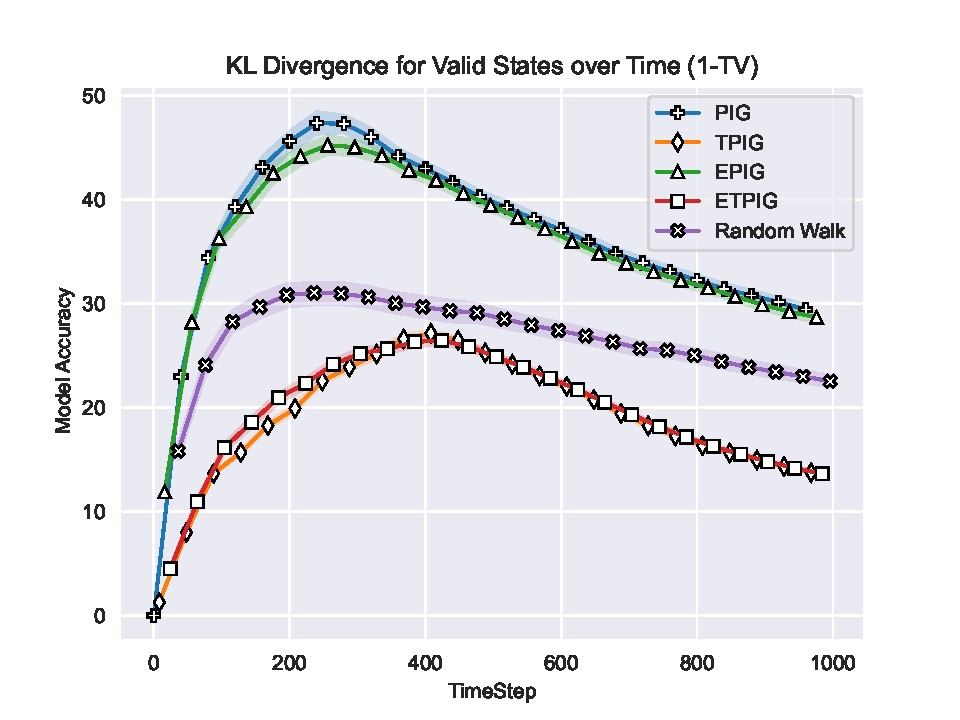
\includegraphics[scale=0.8]{"images/Model_Accuracy_1-TV.pdf"}
	\end{center}
	\caption{Model Accuracy of all Five Policies for 1-TV simulation.}
	\label{Fig:MAFP1TV}
\end{figure}

\begin{figure}[p]
	\begin{center}
		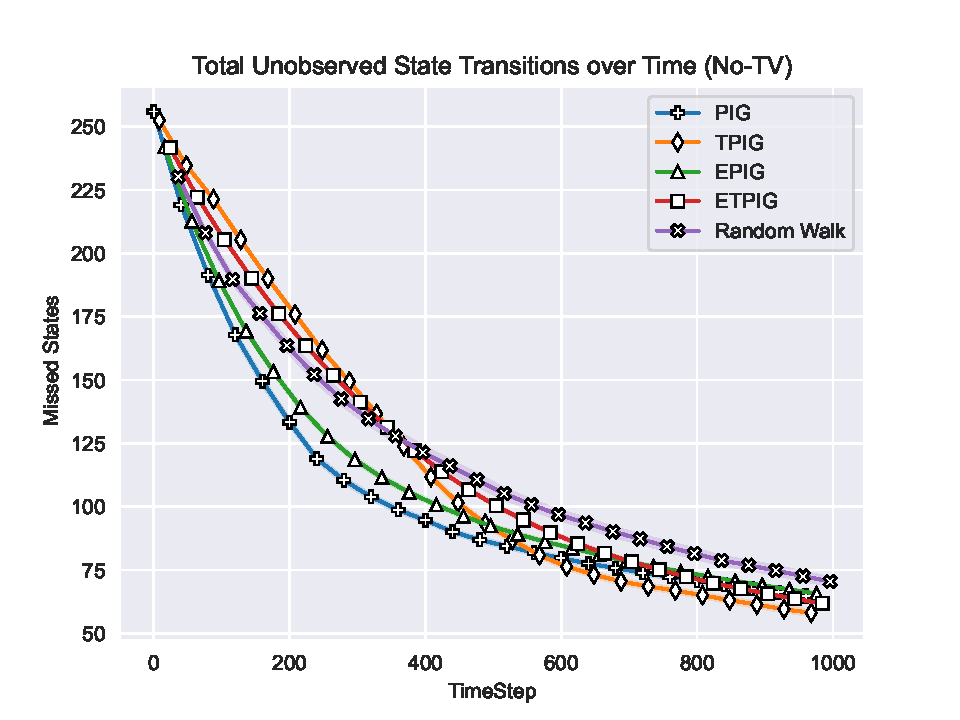
\includegraphics[scale=0.8]{"images/Missed_States_No-TV.pdf"}
	\end{center}
	\caption{Missed States of all Five Policies for No-TV Simulation}
	\label{Fig:MSFP0TV}
\end{figure}
\begin{figure}
	\begin{center}
		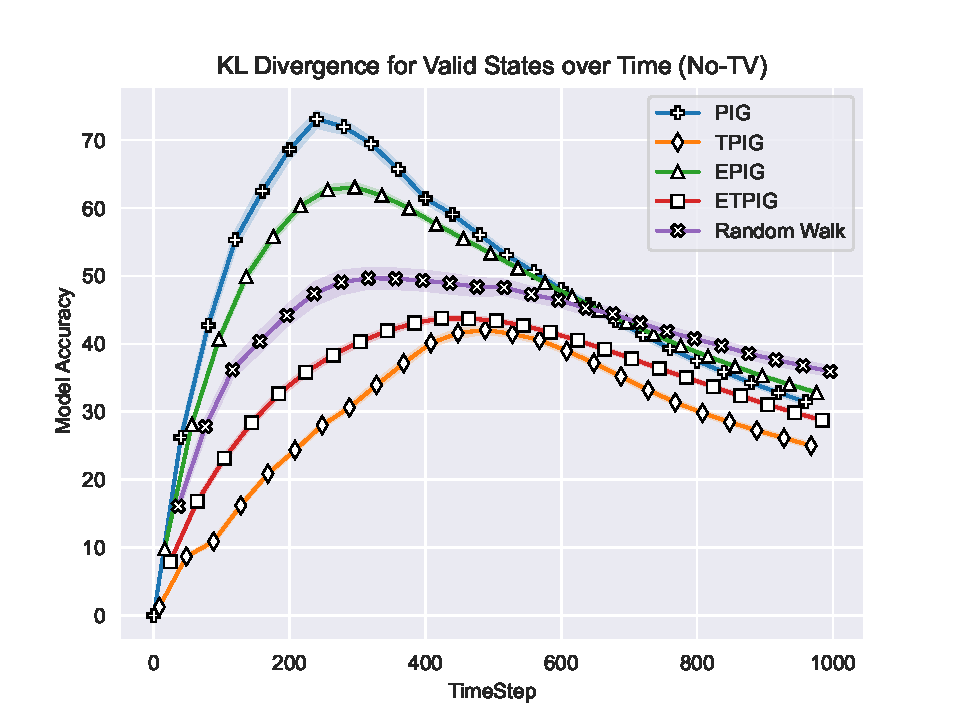
\includegraphics[scale=0.8]{"images/Model_Accuracy_No-TV.pdf"}
	\end{center}
	\caption{Model Accuracy of all Five Policies for No-TV simulation.}
	\label{Fig:MAFP0TV}
\end{figure}




\section{Model Accuracy}
\figurename~\ref{Fig:MAFP4TV}, \ref{Fig:MAFP1TV}, and \ref{Fig:MAFP0TV} are comparisons of the model accuracy of all five policies. This was done through taking the Kullback-Leibler divergence between the policy's model and the true model. Since the Kullback-Leibler divergence returns infinity in the case where a state is in the true model but not the policy's model, these values were ignored and replaced with 0's in the calculations. Lower values are better, but every missing state would add to the KL-divergence if it was found.

Compared to the Random Walk baseline, the PIG algorithm had a worse model accuracy initially in all three simulations. However, since the PIG algorithm had more states known at each of these times as shown in \figurename~\ref{Fig:MSFP4TV}, \ref{Fig:MSFP1TV}, and \ref{Fig:MSFP0TV} PIG and Random Walk have similar model accuracy. At the end of the simulation, however, the results were as follows:

For the 4-TV simulation, (\figurename~\ref{Fig:MAFP4TV}) PIG performed worse than the Random Walk baseline, since it had equivocal KL-divergences, but fewer states explored. For the 1-TV simulation, (\figurename~\ref{Fig:MAFP1TV}) it is hard to determine whether PIG or the Random Walk baseline is better, since PIG had a worse KL-divergence, but had discovered more states. For the No-TV simulation, (\figurename~\ref{Fig:MAFP0TV}) PIG performed better than the Random Walk baseline since it had a better KL-divergence and had discovered more states.

In contrast, the TPIG algorithm had a better model accuracy than both the PIG and Random Walk algorithms for all time-steps. This is particularly notable since the TPIG algorithm surpassed both the PIG and Random Walk algorithm in terms of states found. This means that TPIG had a better Model Accuracy than both PIG and Random Walk while also having explored faster.

The $\epsilon$-greedy implementations performed equally well to the base algorithms for large amounts of time. There was a small increase in performance for EPIG over PIG, but ETPIG had no notable improvement over TPIG for large values of time. In the case of the No-TV simulation, ((\figurename~\ref{Fig:MAFP0TV})) the $\epsilon$-greedy implementations performed worse than the base algorithms. This is expected, as the random nature of $\epsilon$ assists with avoiding Noisy states, but also distracts from regular exploration. When there are no Noisy-TV states, the random nature of $\epsilon$ is a detriment to exploration.



\section{Epsilon Values}
The effect of different values for $\epsilon$ is shown in the following set of graphs. \figurename~\ref{Fig:DREC4TV} through \figurename~\ref{Fig:EAEC0TV} show how $\epsilon$ values affect the EPIG and ETPIG algorithms. Epsilon values were tested in increments of 20\%.
\begin{figure}
	\begin{center}
		\subfloat[4-TV EPIG Simulation \label{Fig:DRECEP4TV}]{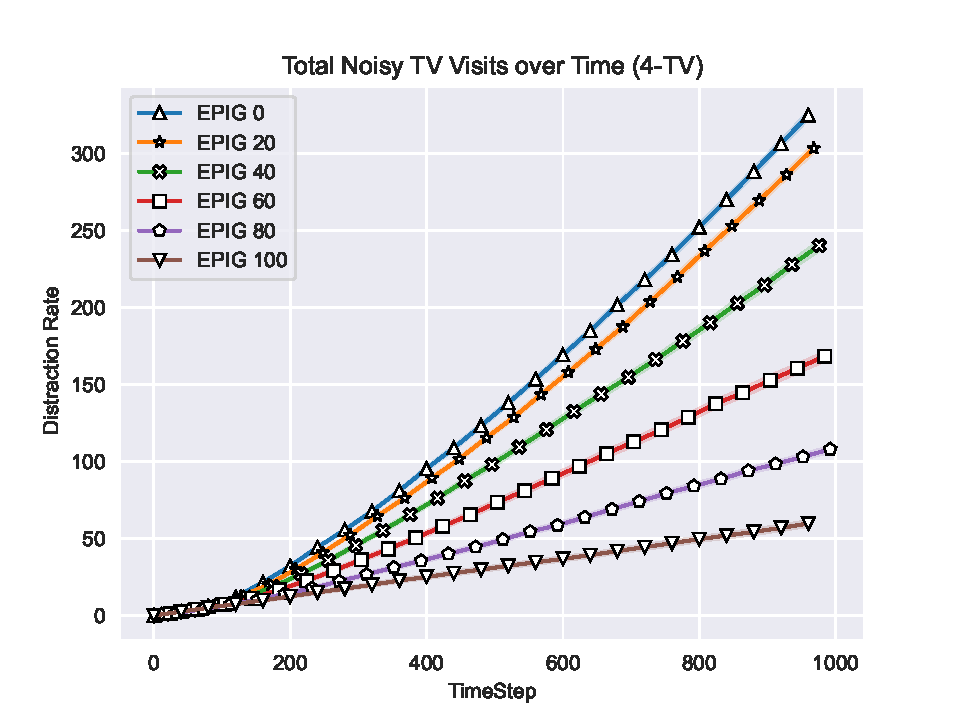
\includegraphics[scale=0.8]{"images/Epsilon_Distractions_EPIG_4-TV.pdf"}}\hfill
		
		\subfloat[4-TV ETPIG Simulation \label{Fig:DRECET4TV}]{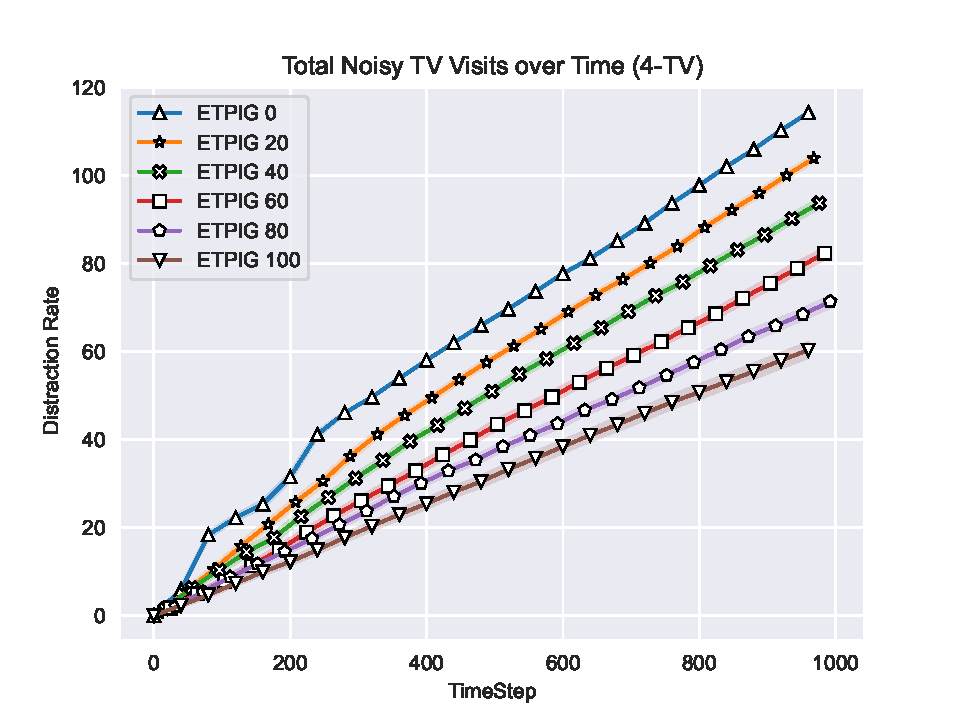
\includegraphics[scale=0.8]{"images/Epsilon_Distractions_ETPIG_4-TV.pdf"}}\hfill
	\end{center}
	\caption{Distraction Rate Epsilon Comparison EPIG VS ETPIG 4-TV Simulation}
	\label{Fig:DREC4TV}
\end{figure}

\begin{figure}	
	\begin{center}
		\subfloat[1-TV EPIG Simulation \label{Fig:DRECEP1TV}]{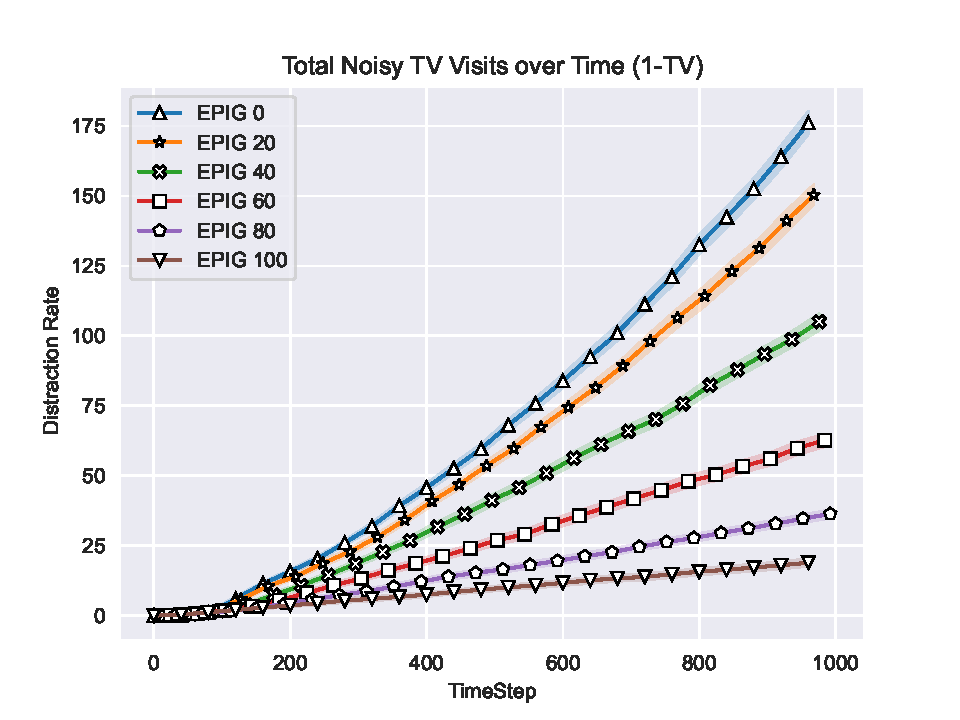
\includegraphics[scale=0.8]{"images/Epsilon_Distractions_EPIG_1-TV.pdf"}}\hfill
		
		\subfloat[1-TV ETPIG Simulation \label{Fig:DRECET1TV}]{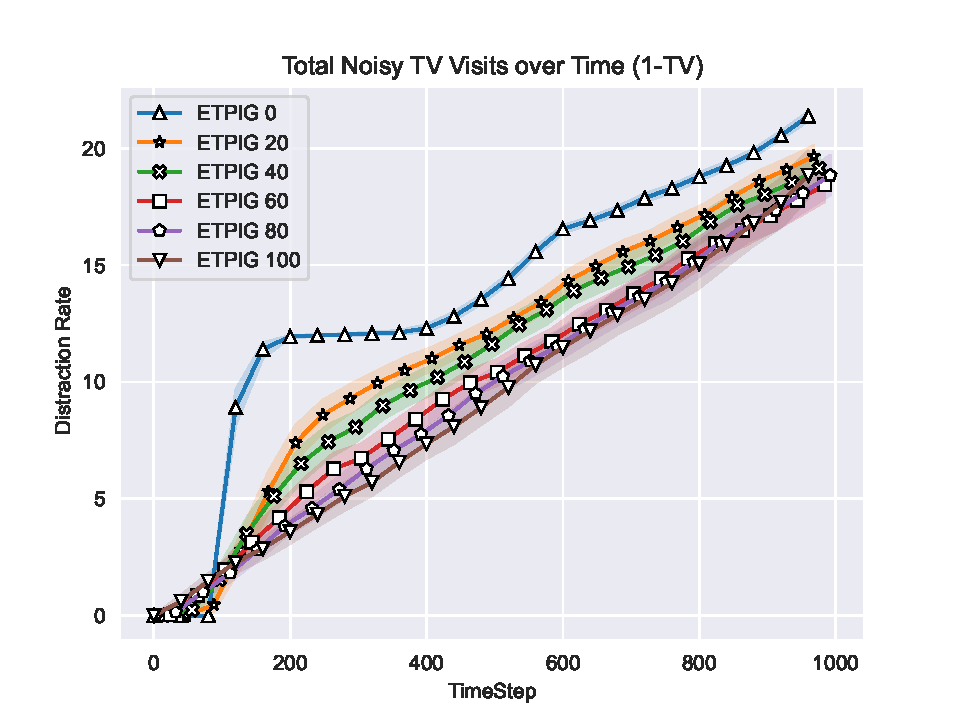
\includegraphics[scale=0.8]{"images/Epsilon_Distractions_ETPIG_1-TV.pdf"}}\hfill
	\end{center}
	\caption{Distraction Rate Epsilon Comparison EPIG VS ETPIG 1-TV Simulation}
	\label{Fig:DREC1TV}
\end{figure}

\begin{figure}	
	\begin{center}
		\subfloat[No-TV EPIG Simulation \label{Fig:DRECEP0TV}]{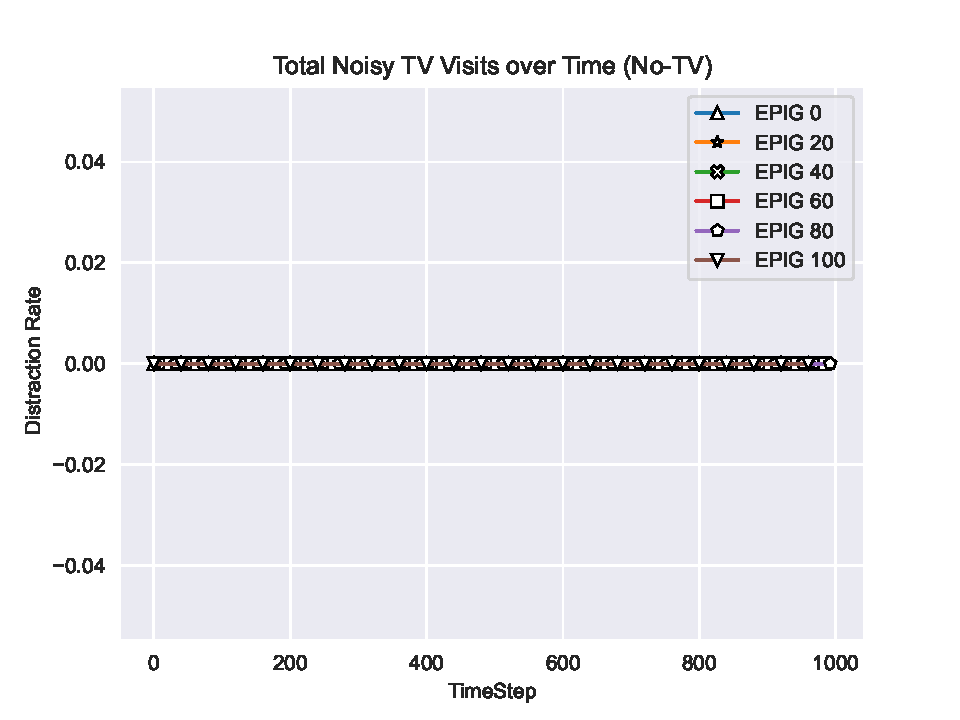
\includegraphics[scale=0.8]{"images/Epsilon_Distractions_EPIG_No-TV.pdf"}}\hfill
		
		\subfloat[No-TV ETPIG Simulation \label{Fig:DRECET0TV}]{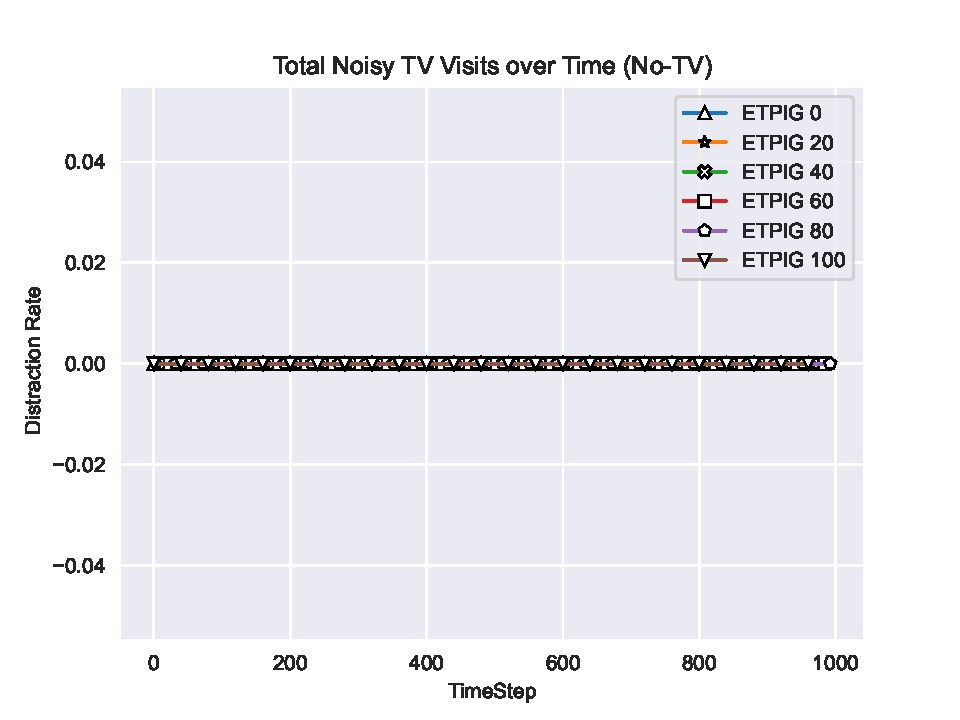
\includegraphics[scale=0.8]{"images/Epsilon_Distractions_ETPIG_No-TV.pdf"}}\hfill
	\end{center}	
	\caption{Distraction Rate Epsilon Comparison EPIG VS ETPIG No-TV Simulation}
	\label{Fig:DREC0TV}
\end{figure}


\subsection{Distraction Rate}
In the 4-TV simulation, (\figurename~\ref{Fig:DREC4TV}) The distraction rate decreases as $\epsilon$ increases. This is true in both for EPIG and ETPIG. In EPIG, (\figurename~\ref{Fig:DRECEP4TV}) as $\epsilon$ increases towards 100\% not only does the rate of distraction decrease but the frequency of distraction decreases as well. This is expected behavior, as the more random the algorithm is, the less often it should tend towards its biases, in this case the Noisy-TV.

In ETPIG, (\figurename~\ref{Fig:DRECET4TV}) the initial rate of distraction is affected by the value of $\epsilon$, but the frequency of distraction is unaffected (Or affected much less). There are some weird artifacts in the case of $\epsilon = 0$, also known as the TPIG case. This suggests that adding some randomness to the TPIG algorithm smooths out some irregular behavior.

In the 1-TV simulation, (\figurename~\ref{Fig:DREC1TV}) the distraction rate decreases as $\epsilon$ increases. This is true for both EPIG and ETPIG. The results for EPIG (\figurename~\ref{Fig:DRECEP1TV}) in the 1-TV simulation are very similar to the 4-TV simulation results. Both the distraction rate and frequency of distraction decrease as $\epsilon$ increases.

In ETPIG, (\figurename~\ref{Fig:DRECET1TV}) however, the results are slightly different for the 1-TV simulation compared to the 4-TV simulation. Unlike the 4-TV simulation, in the 1-TV simulation, the distraction rate and frequency for the ETPIG algorithm approach towards the Random Walk algorithm ($\epsilon = 100$). This is very interesting, as it suggests that the ETPIG algorithm has figured out the Noisy-TV's and is now avoiding them, performing better than the Random Walk baseline. Around time-step 100, there is a point when all the ETPIG policies pivot. This suggests that ETPIG may perform worse for smaller amounts of time when it has a low value of $\epsilon$. There are still weird artifacts in the case of $\epsilon = 0$, with TPIG performing much worse initially than its ETPIG counterpart. Similarly, TPIG does not appear to converge to the Random Walk algorithm, unlike its $\epsilon$-greedy counterpart ETPIG. Whether this is true for large time-steps or not cannot be determined without longer simulations. 

In the No-TV simulation, (\figurename~\ref{Fig:DREC0TV}) there is no Noisy-TV to distract any of the algorithms. As such, all the algorithms perform equally well on this metric and are never distracted. This makes the graph a flat line.
\begin{figure}
	\begin{center}
		\subfloat[4-TV EPIG Simulation \label{Fig:EMECEP4TV}]{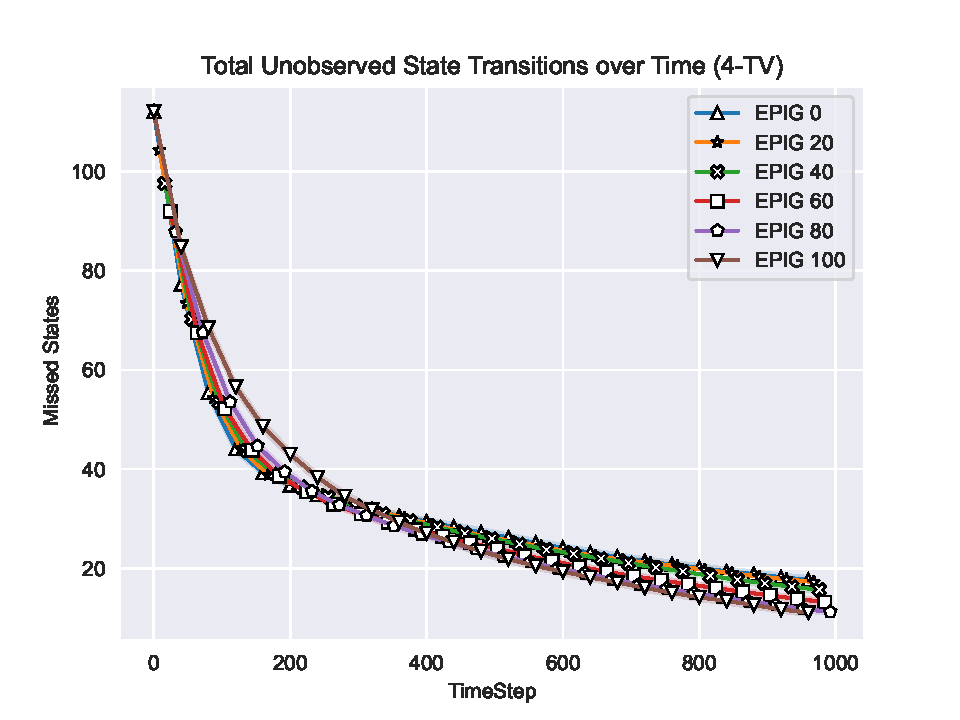
\includegraphics[scale=0.8]{"images/Epsilon_Missed_States_EPIG_4-TV.pdf"}}\hfill
			
		\subfloat[4-TV ETPIG Simulation \label{Fig:EMECET4TV}]{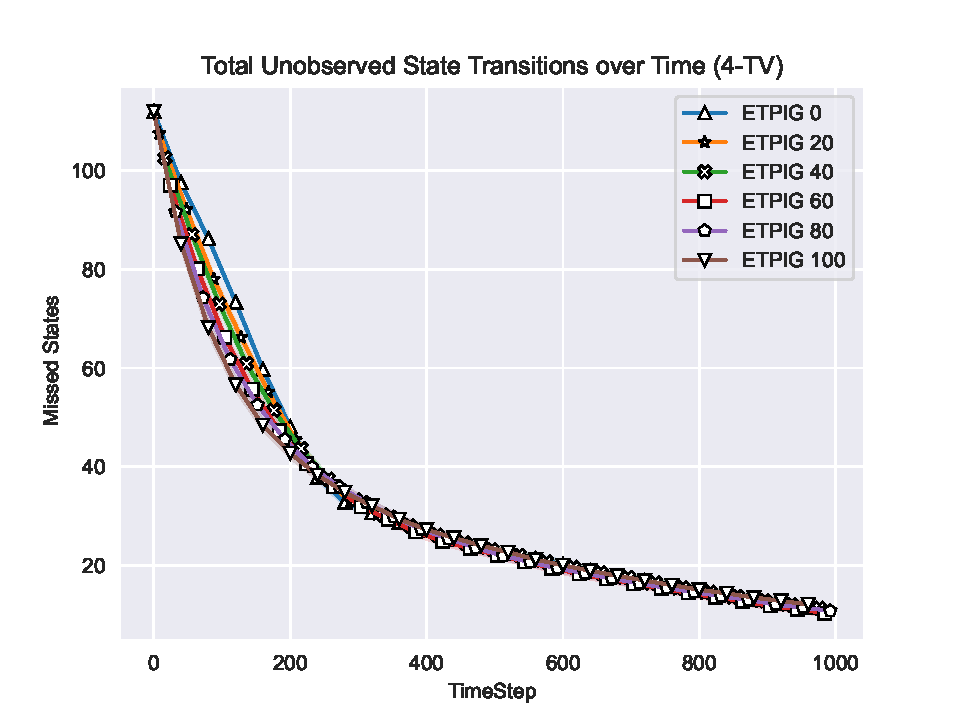
\includegraphics[scale=0.8]{"images/Epsilon_Missed_States_ETPIG_4-TV.pdf"}}\hfill
	\end{center}
	\caption{Missed States Epsilon Comparison EPIG VS ETPIG 4-TV Simulation}
	\label{Fig:EMEC4TV}
\end{figure}

\begin{figure}
	\begin{center}
		\subfloat[1-TV EPIG Simulation \label{Fig:EMECEP1TV}]{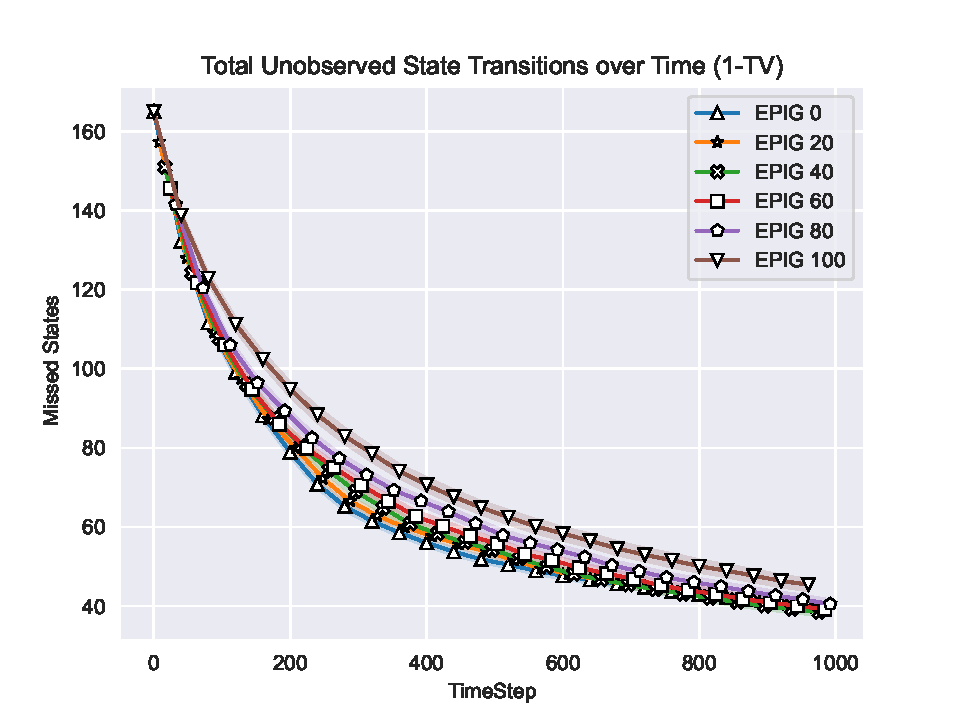
\includegraphics[scale=0.8]{"images/Epsilon_Missed_States_EPIG_1-TV.pdf"}}\hfill
		\subfloat[1-TV ETPIG Simulation \label{Fig:EMECET1TV}]{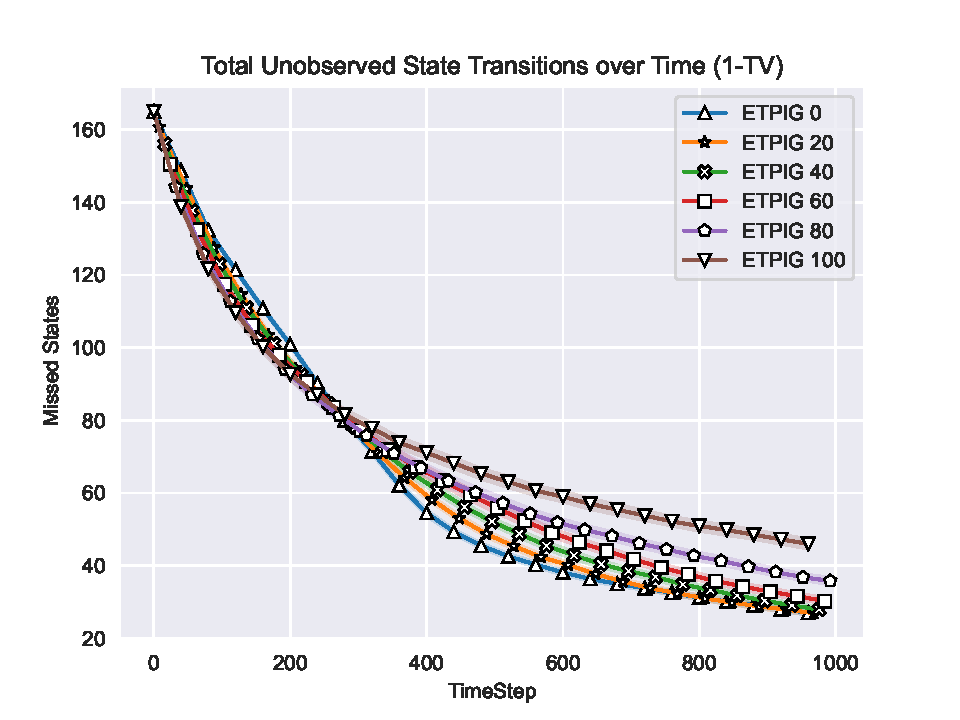
\includegraphics[scale=0.8]{"images/Epsilon_Missed_States_ETPIG_1-TV.pdf"}}\hfill
	\end{center}
	\caption{Missed States Epsilon Comparison EPIG VS ETPIG 1-TV Simulation}
	\label{Fig:EMEC1TV}
\end{figure}

\begin{figure}
	\begin{center}
		\subfloat[No-TV EPIG Simulation \label{Fig:EMECEP0TV}]{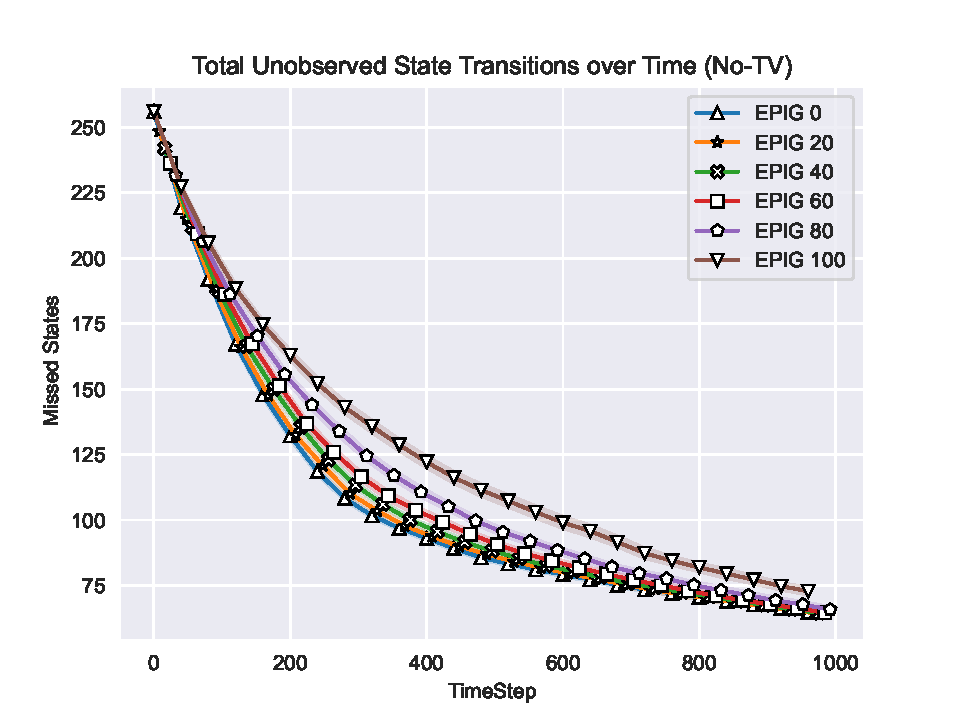
\includegraphics[scale=0.8]{"images/Epsilon_Missed_States_EPIG_No-TV.pdf"}}\hfill
			
		\subfloat[No-TV ETPIG Simulation \label{Fig:EMECET0TV}]{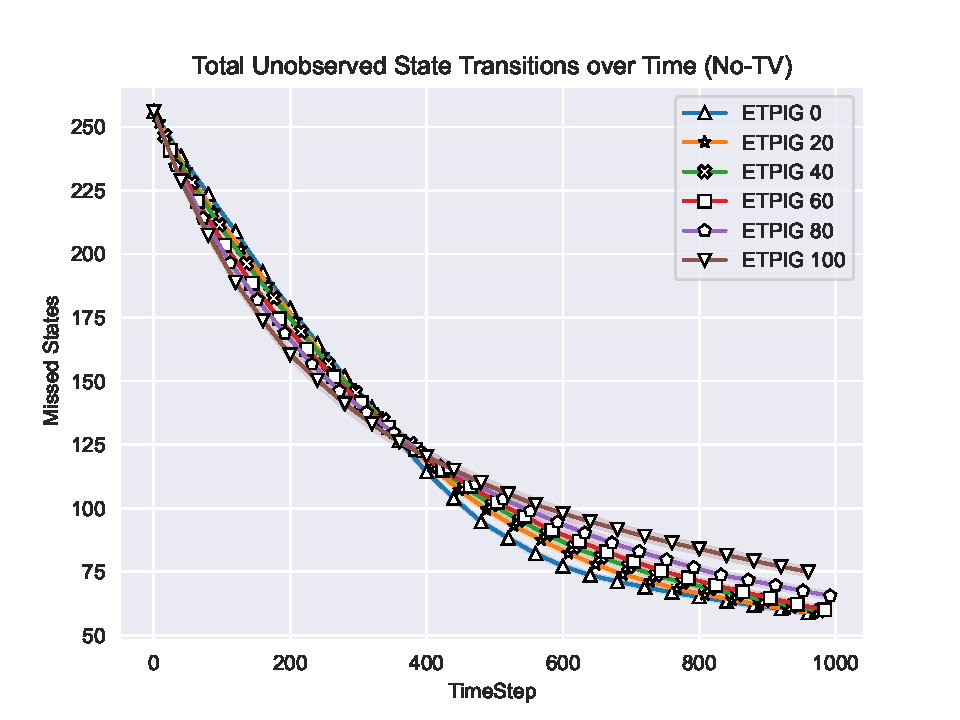
\includegraphics[scale=0.8]{"images/Epsilon_Missed_States_ETPIG_No-TV.pdf"}}\hfill
	\end{center}
	\caption{Missed States Epsilon Comparison EPIG VS ETPIG No-TV Simulation}
	\label{Fig:EMEC0TV}
\end{figure}

\subsection{Learning Rate}
In the 4-TV simulation, (\figurename~\ref{Fig:EMEC4TV}) higher values of $\epsilon$ generally provided better results than lower values of $\epsilon$. In the case of EPIG, (\figurename~\ref{Fig:EMECEP4TV}) although higher values of $\epsilon$ performed worse initially, they performed better than low values of $\epsilon$ after around time step 350. On the contrary, lower values of $\epsilon$ fell off at around the same point, performing worse in the end.

In ETPIG, (\figurename~\ref{Fig:EMECET4TV}) however, high values of $\epsilon$ performed better throughout the entire simulation. Low values of $\epsilon$ performed worse initially, but approached and matched the performance of high $\epsilon$ values at around time step 250. From that time onward, all values of $\epsilon$ seem to perform roughly equally.

In the 1-TV simulation, (\figurename~\ref{Fig:EMEC1TV}) the results were significantly different from those of the 4-TV simulation. Low values of $\epsilon$ performed better for both EPIG and ETPIG in the 1-TV simulation than their high $\epsilon$ valued counterparts. In the case of EPIG, (\figurename~\ref{Fig:EMECEP1TV}) low values of $\epsilon$ performed better than high values of $\epsilon$ for the entire simulation. High values of $\epsilon$ do tend to approach lower values of $\epsilon$ as the simulation continues, but to determine whether they converge or not would require longer simulations.

In ETPIG, (\figurename~\ref{Fig:EMECET1TV}) however, low values of $\epsilon$ performed worse initially, but surpassed high values of $\epsilon$ around time step 300. Unlike in the 4-TV simulation, in the 1-TV simulation, ETPIG is clearly better with lower values of $\epsilon$ towards later time steps.

In the No-TV simulation, (\figurename~\ref{Fig:EMEC0TV}) the results were very similar to those of the 1-TV simulation. In the case of EPIG, (\figurename~\ref{Fig:EMECEP0TV}) although the scales are different (As expected of two simulations of different size), the relationships between the different values of $\epsilon$ and how their graphs behave were nearly identical.

In ETPIG, (\figurename~\ref{Fig:EMECET0TV}) a similar thing is true. The results for ETPIG in the 1-TV and No-TV simulations are extremely similar, with the main difference being the time step when the graph pivots and low values of $\epsilon$ becomes better than high values of $\epsilon$. This change is probably a result of the simulation size changing, as the crossover point shifts forward in time as the size of the simulation increases. In simulation 4-TV, this point is at time step 200, while it is at time step 300 in simulation 1-TV and time step 400 in simulation No-TV. Further testing would be required to determine this for sure.
\begin{figure}
	\begin{center}
		\subfloat[4-TV EPIG Simulation \label{Fig:EAECEP4TV}]{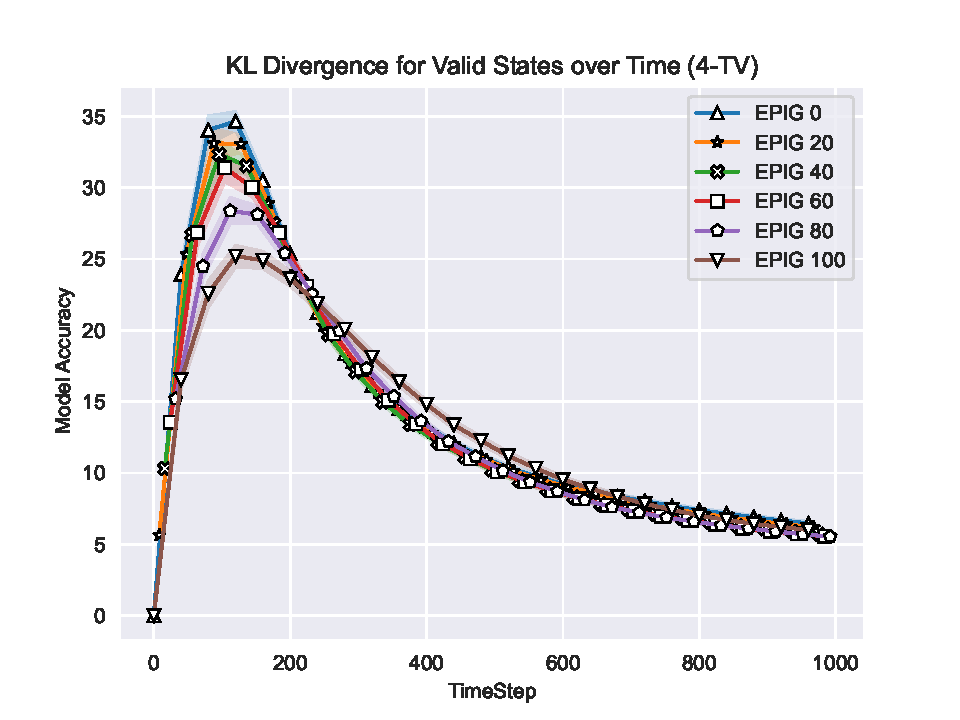
\includegraphics[scale=0.8]{"images/Epsilon_Model_Accuracy_EPIG_4-TV.pdf"}}\hfill
		\subfloat[4-TV ETPIG Simulation \label{Fig:EAECET4TV}]{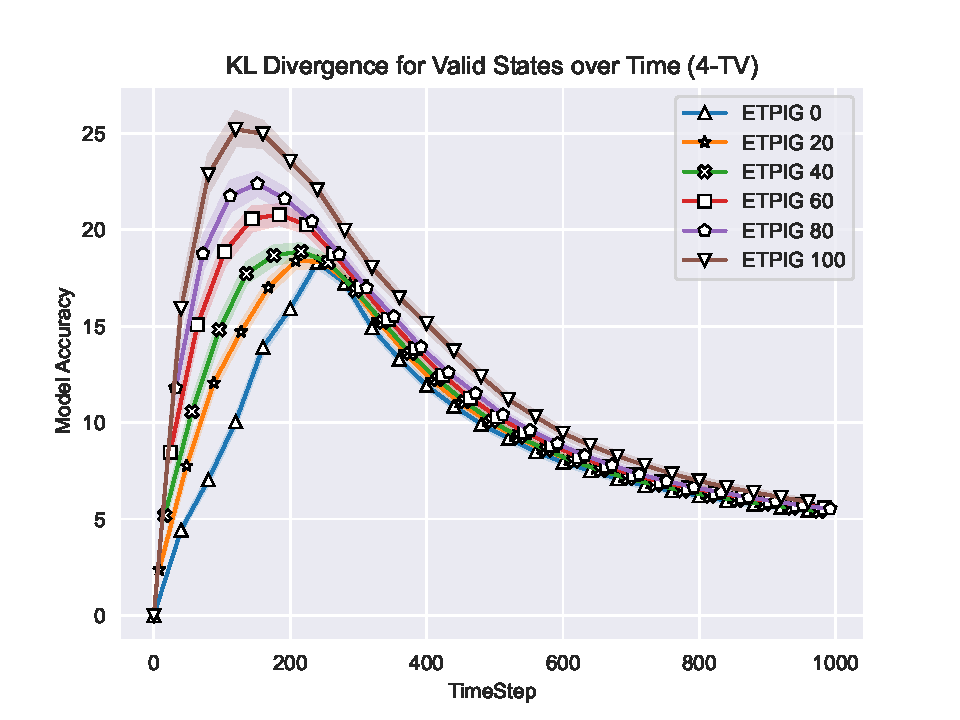
\includegraphics[scale=0.8]{"images/Epsilon_Model_Accuracy_ETPIG_4-TV.pdf"}}\hfill
	\end{center}
	\caption{Model Accuracy Epsilon Comparison EPIG VS ETPIG 4-TV Simulation}
	\label{Fig:EAEC4TV}
\end{figure}

\begin{figure}
	\begin{center}
		\subfloat[1-TV EPIG Simulation \label{Fig:EAECEP1TV}]{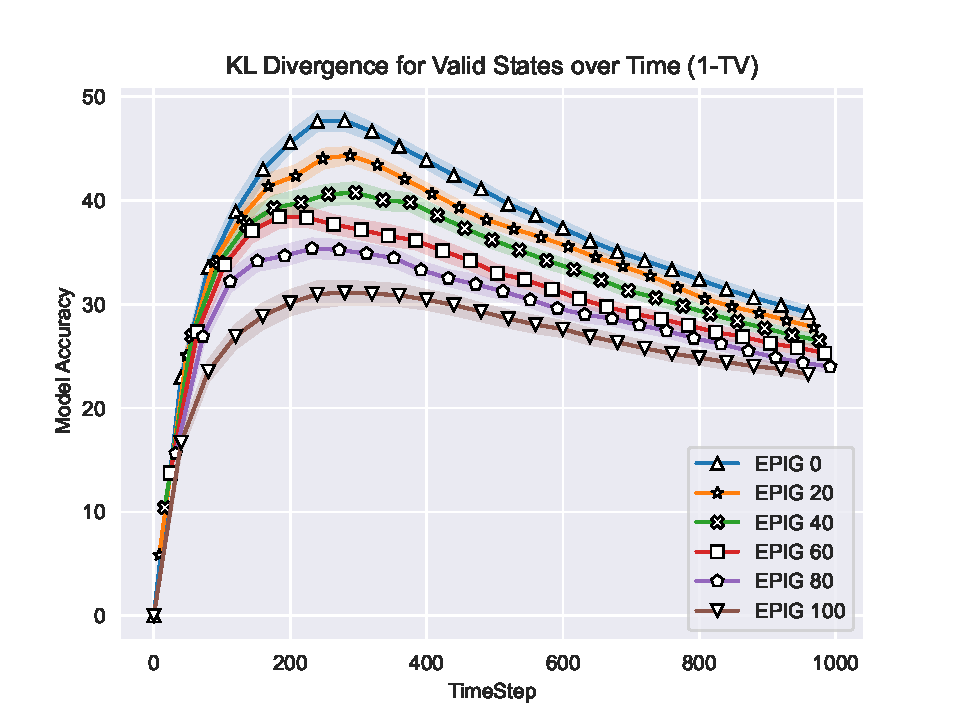
\includegraphics[scale=0.8]{"images/Epsilon_Model_Accuracy_EPIG_1-TV.pdf"}}\hfill
		\subfloat[1-TV ETPIG Simulation \label{Fig:EAECET1TV}]{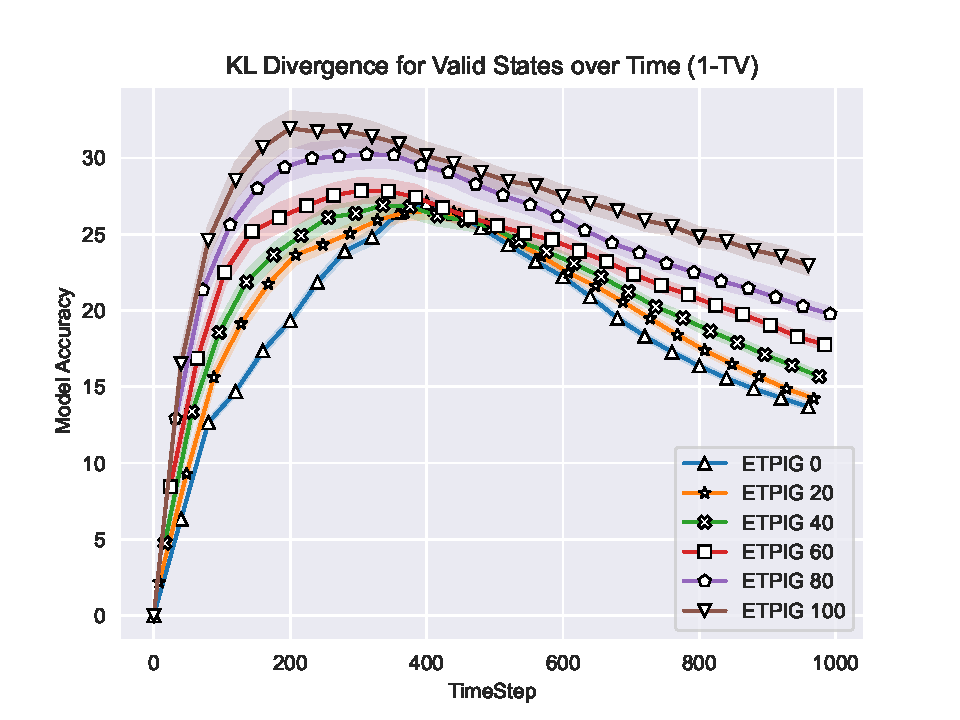
\includegraphics[scale=0.8]{"images/Epsilon_Model_Accuracy_ETPIG_1-TV.pdf"}}\hfill
	\end{center}
	\caption{Model Accuracy Epsilon Comparison EPIG VS ETPIG 1-TV Simulation}
	\label{Fig:EAEC1TV}
\end{figure}

\begin{figure}
	\begin{center}
		\subfloat[No-TV EPIG Simulation \label{Fig:EAECEP0TV}]{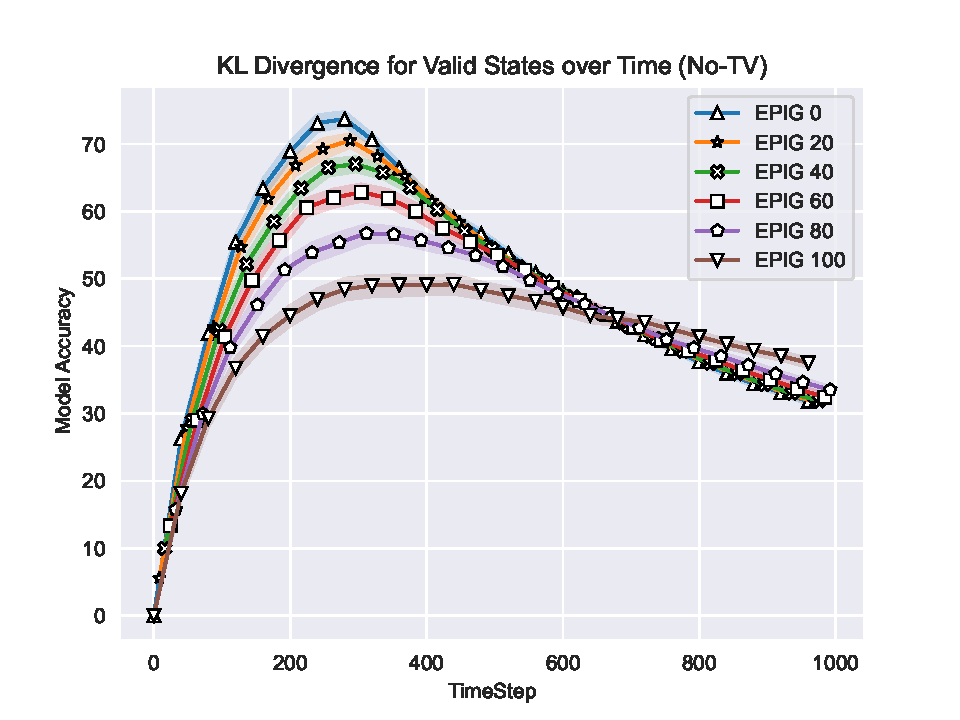
\includegraphics[scale=0.8]{"images/Epsilon_Model_Accuracy_EPIG_No-TV.pdf"}}\hfill
		\subfloat[No-TV ETPIG Simulation \label{Fig:EAECET0TV}]{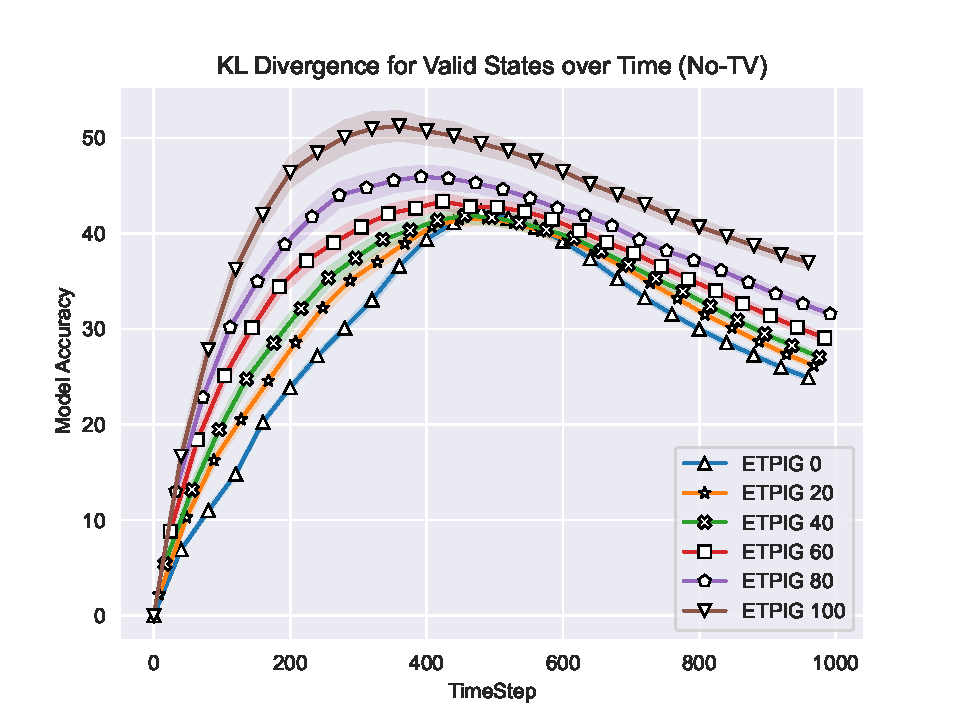
\includegraphics[scale=0.8]{"images/Epsilon_Model_Accuracy_ETPIG_No-TV.pdf"}}\hfill
	\end{center}
	\caption{Model Accuracy Epsilon Comparison EPIG VS ETPIG No-TV Simulation}
	\label{Fig:EAEC0TV}
	
\end{figure}
\subsection{Model Accuracy}
As a metric, the Kullback-Leibler divergence alone cannot provide an accurate measurement. This is because the Kullback-Leibler divergence returns an infinity whenever a state transition is in the true distribution, but not in the agent's model. To allow for any visible results on this metric, I have replaced all of these infinities with 0 when taking these measurements. As such, the summation for the Kullback-Leibler divergence has a different number of elements depending on the number of state transitions found by the agent. To provide any meaningful analysis, the Kullback-Leibler divergence is used in conjunction with the learning rate discussed in the previous section. Every explored state adds a positive value to the KL-divergence total. As such, if two agents had the same Kullback-Leibler divergence with the true distribution $\Theta$ but agent 1 had discovered more states than agent 2, than agent 1 performed better than agent 2.

In the 4-TV simulation, (\figurename~\ref{Fig:EAEC4TV}) higher values of $\epsilon$ had a worse performance than lower values of $\epsilon$. In the case of EPIG, (\figurename~\ref{Fig:EAECEP4TV}) middle values of $\epsilon$ had better KL-divergences than both high and low values of $\epsilon$. Although high values of $\epsilon$ performed better initially, they performed worse for larger values of time. In addition, since high values of $\epsilon$ performed worse than low values of $\epsilon$ for the related learning rate metric, high values of $epsilon$ performed worse than it appears, being roughly equivocal to the other values of $\epsilon$ in the beginning time steps. Towards the simulation's end, although high values of $\epsilon$ had a worse KL-divergence, they had discovered more states then the other values of $\epsilon$ making them equivocal if not better. 

Low values of $\epsilon$ had a worse KL-divergence initially, but rapidly converged to the other values of $\epsilon$ in the middle stages of time before falling off towards the end of the simulation. Since low values of $\epsilon$ performed well initially with respect to learning rate before falling off and performing the worst towards the end of the simulation, we can determine that low values of $\epsilon$ performed equivocal to the other values of $\epsilon$ at the start of the simulation, but performed the worst of all the $epsilon$ values by the end.

%In short, for EPIG in the 4-TV simulation, high values of $\epsilon$ are equivocal to middle values of $\epsilon$, while low values of $\epsilon$ performed badly.

In ETPIG, (\figurename~\ref{Fig:EAECET4TV}) however, low values of $\epsilon$ remained better than high values of $\epsilon$ for the entire simulation. At the beginning of the simulation, lower values of $\epsilon$ had a worse learning rate, making their KL-divergence performance equivocal to the other $\epsilon$ values. However, the learning rate for all the $\epsilon$ values converge around time step 200. Since low values of $\epsilon$ still have the lowest KL-divergence of all the $\epsilon$'s after time step 200, in the 4-TV simulation lower values of $\epsilon$ have better performance than higher values of $\epsilon$ for the ETPIG algorithm.

In the 1-TV simulation, (\figurename~\ref{Fig:EAEC1TV}) $\epsilon$ had different effects on EPIG and ETPIG. In the case of EPIG, (\figurename~\ref{Fig:EAECEP1TV}) higher values of $\epsilon$ performed better and had lower KL-divergences than lower values of $\epsilon$. However, since the learning rate of performed inverse to this, (where high values of $\epsilon$ performed worse than low values of $\epsilon$), the KL-divergences among the different values of $\epsilon$ for EPIG are equivocal to each other.

In ETPIG, (\figurename~\ref{Fig:EAECET1TV}) however, the lower values of $\epsilon$ performed better than the higher values of $\epsilon$ for the entire simulation. The learning rate of ETPIG in the 1-TV simulation performs better for high values of $\epsilon$ than low values of $\epsilon$ before time step 300. After that point, low values of $\epsilon$ perform better than high values of $\epsilon$. This means that the KL-divergences of ETPIG for simulation 1-TV are equivocal up to time step 300. After this point, lower values of $\epsilon$ perform better than high values of $\epsilon$.

%In short, for PIG all values of $\epsilon$ are roughly equal, while for ETPIG low values of $\epsilon$ perform equal or better than higher values of $\epsilon$ in simulation 1-TV.

In the No-TV simulation, (\figurename~\ref{Fig:EAEC0TV}) lower values of $\epsilon$ generally provided better results than higher values of $\epsilon$. In the case of EPIG, (\figurename~\ref{Fig:EAECEP0TV}) lower values of $\epsilon$ initially had worse results than higher values of $\epsilon$. However, as the learning rate for EPIG in the No-TV simulation was faster for low values of $\epsilon$ than high values of $epsilon$, the value of the KL-divergences for EPIG are equivocal. Around time step 600, the KL-divergence of the low values of $\epsilon$ becomes better than that of the high values of $\epsilon$. Since the learning rate of EPIG for simulation No-TV is better for the entire simulation, the KL-divergence of low value $\epsilon$ EPIG after time step 600 is better than that of high value $\epsilon$ EPIG. Whether this changes again at further time steps would require a longer simulation to determine.


In ETPIG, (\figurename~\ref{Fig:EAECET0TV}) on the other hand, lower values of $\epsilon$ have a better KL-divergence than higher values of $\epsilon$ for the entire No-TV simulation. The learning rate of ETPIG for the No-TV simulation is better for high values of $\epsilon$ than lower values of $\epsilon$ up to around time step 350. This means that the KL-divergences of ETPIG for low and high values of $\epsilon$ are equivocal until time step 350. After time step 350, lower values of $\epsilon$ have better KL-divergences and faster learning rates than higher values of $\epsilon$.

%In short, in both EPIG and ETPIG lower values of $\epsilon$ perform roughly equal or better than high values of $\epsilon$ for the No-TV simulation.



\chapter{Conclusions}
The TPIG algorithm performed better than the PIG algorithm in all three metrics. TPIG was distracted by the Noisy-TV less than PIG. TPIG was able to explore and find new states faster than PIG was. TPIG was able to model the true distribution $\Theta$ more closely than PIG. For short simulations, PIG may explore faster than TPIG, but TPIG approaches a complete exploration faster than PIG does.
\section{Future Work}
There is definitely more potential in this area of research. Information theory has already been utilized in reinforcement learning, but directly learning based on the measurement of information found in the environment has great potential. 

Some areas of future research include:
\begin{itemize}
	\item Trying other reinforcement learning methods such as Monte Carlo or n-step temporal difference on information gain.
	\item The KL-divergence metric had some drastic flaws due to how it interacted with infinity. Future work could adapt the KL-divergence into a mean squared error of the individual states instead of a sum. This could potentially provide a better metric for future analysis.
	\item Better code implementations of the algorithms in this paper could allow for time-complexity comparisons instead of comparisons over time-steps.
	\item Further variety in simulations and more in-depth analysis of how simulation size affects TPIG.
	\item Expanding the starting state to a set of starting states, or use of multiple similar simulations could be used to test knowledge transfer to similar tasks.
	\item Expanding current formulae to work with continuous environments.
	\item Comparing TPIG with other reinforcement learning algorithms in both environments with and without Noisy-TV's
	\item Adapting TPIG to work with both external and internal reward.
\end{itemize}

Alternative methods of resisting noise should also be looked into. One method that seemed promising but outside the scope of this paper, involved clustering state transitions together. A ``blurring" layer would be added between the observed state and the policy used to pick an action. This ``blurring" layer creates the smallest mask that it can such that every observed state transition has been visited at least $n$ times. Initially, this method would blur all states to look like a single state. As the agent continues to explore, however, similar state transitions (or repeated transitions) will be grouped together by the ``blurring" layer. This means that the agent will naturally group noisy states (which tend to be unique from other states) together. Well explored areas will have their own clusters while new areas will be merged together into an ``unknown" area to explore. An advantage of this method is it could theoretically work with any underlying policy since it manipulates how the agent perceives the environment, rather than the agent's decision process.

\section{Closing Thoughts}
TPIG is a step towards making algorithms more robust to external noise. External noise is a big problem that needs to be addressed with any potential real-world implementation of reinforcement learning methods. Hopefully this paper will spark more interest into this important and underdeveloped area of research.

%\chapter{Appendix A}

%\begin{comment}
%\chapter{Previous Work}
%
%
%There has been a lot of previous work that is not at all like my work.
%For example,
%% The following if-then-else allows us to get good results with
%% any bibliography/citation style.
%\ifthesiscitations
%\citeN{Kringle} % if we are using the thesiscitations style
%\else
%Kringle~\cite{Kringle} % if we are using a more primitive citation style
%\fi
%showed that apples and goats have almost
%nothing in common, other than both being red.  The major problem with
%Kringle's study is that he used a goat that had been spray painted
%red, and his apple was a golden delicious variety.  Criticism of
%Kringle's methods has been harsh, and so far, no one has been able to
%replicate his results.
%
%Several researchers have compared trout to
%eagles~\cite{Simmons,Sheppard}.  The consensus that has emerged is
%that they are quite different, and only an idiot would try to eat an
%eagle~\cite{Idiot}.
%
%\chapter{Methods}
%In this chapter, I will present the methods for my comparison, and
%fill in with a lot of gibberish.  For instance, I will say things like
%``Gnats and Gnus come in twos'' in order to fill space and make my
%thesis seem longer than it really is.  This is a tactic used by some
%people to hide the fact that their research is worthless.  The idea is
%that if the thesis is long enough and boring enough, the thesis
%comittee members will go to sleep every time they try to read it.
%
%Another thing that I may do is to use very long words, such as
%onomatopoeia, for no apparent reason.  By employing voluminous
%instances of obfuscatory and expansive vocables, the lack of
%quintessence of this monograph can be adumbrated from all but
%the most erudite, didactic, and scholarly bibliophiles.
%
%
%\chapter{Results}
%My research had fabulous results. I will now tell you about
%the results, because they are the best!  You are not going
%to believe how good my results are.
%
%\section{Visual comparison}
%%\index{comparison!visual}
%
%\begin{table}
%\caption{Results of visual comparison studies.}
%\begin{center}
%  \begin{tabular}{|c|c|}
%    \hline
%    \bf Categories & \bf Percent Correct\\
%    \hline
%    \hline
%    insect/mammal & 76\\
%    \hline
%    gnat/gnu & 69\\
%    \hline
%  \end{tabular}
%\end{center}
%\label{table:comp1}
%\end{table}
%
%The first test that I performed was a visual comparison of gnats and
%gnus.  First, I went on the internet and downloaded several thousand
%pictures of gnats, and one picture of a gnu.  Then, I had two
%volunteers compare them and categorize them as insect
%%\index{insect}
%or mammal.
%%\index{mammal}
%Next, I selected another group of volunteers and
%had them classify the photographs as either gnat or gnu.
%
%
%\begin{sidewaysfigure}
%\begin{center}
%\subfloat{\resizebox{0.45\textheight}{!}{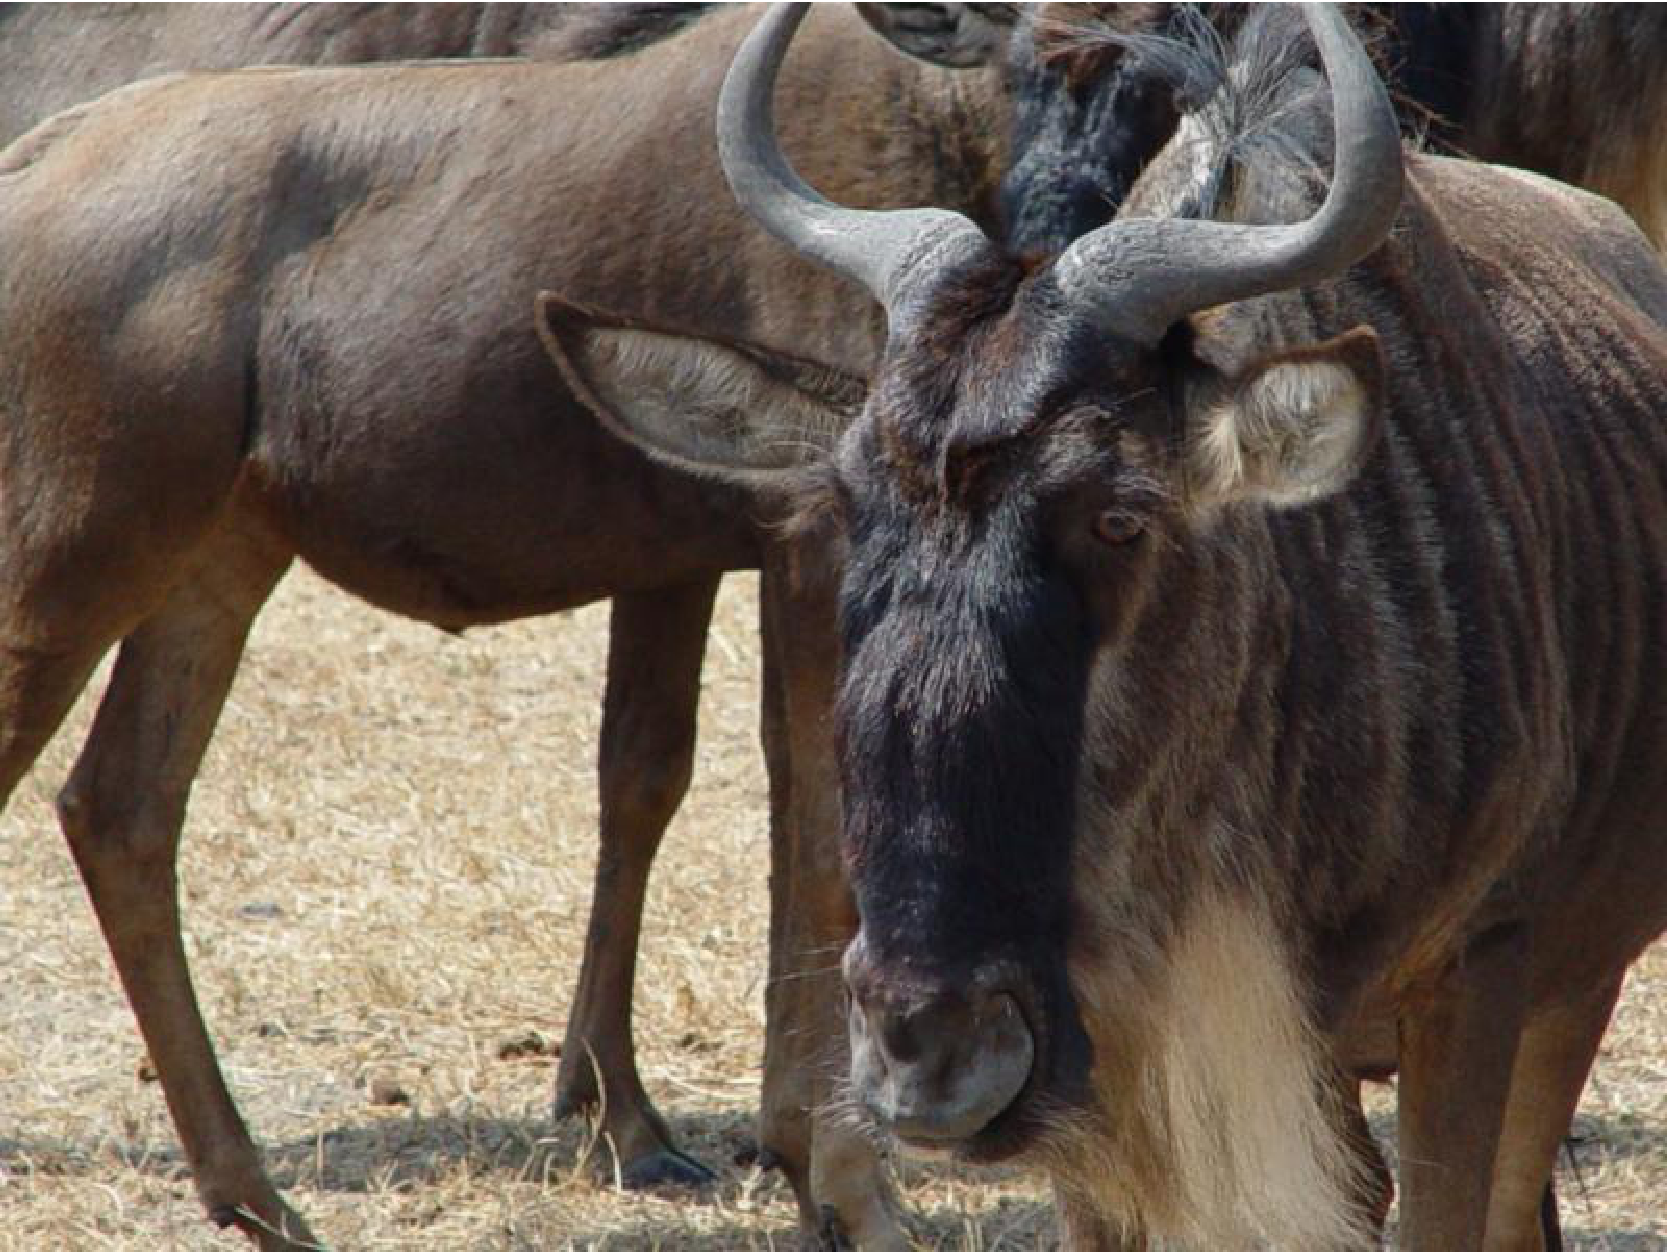
\includegraphics{images/gnu.pdf}}}
%\subfloat{\resizebox{0.45\textheight}{!}{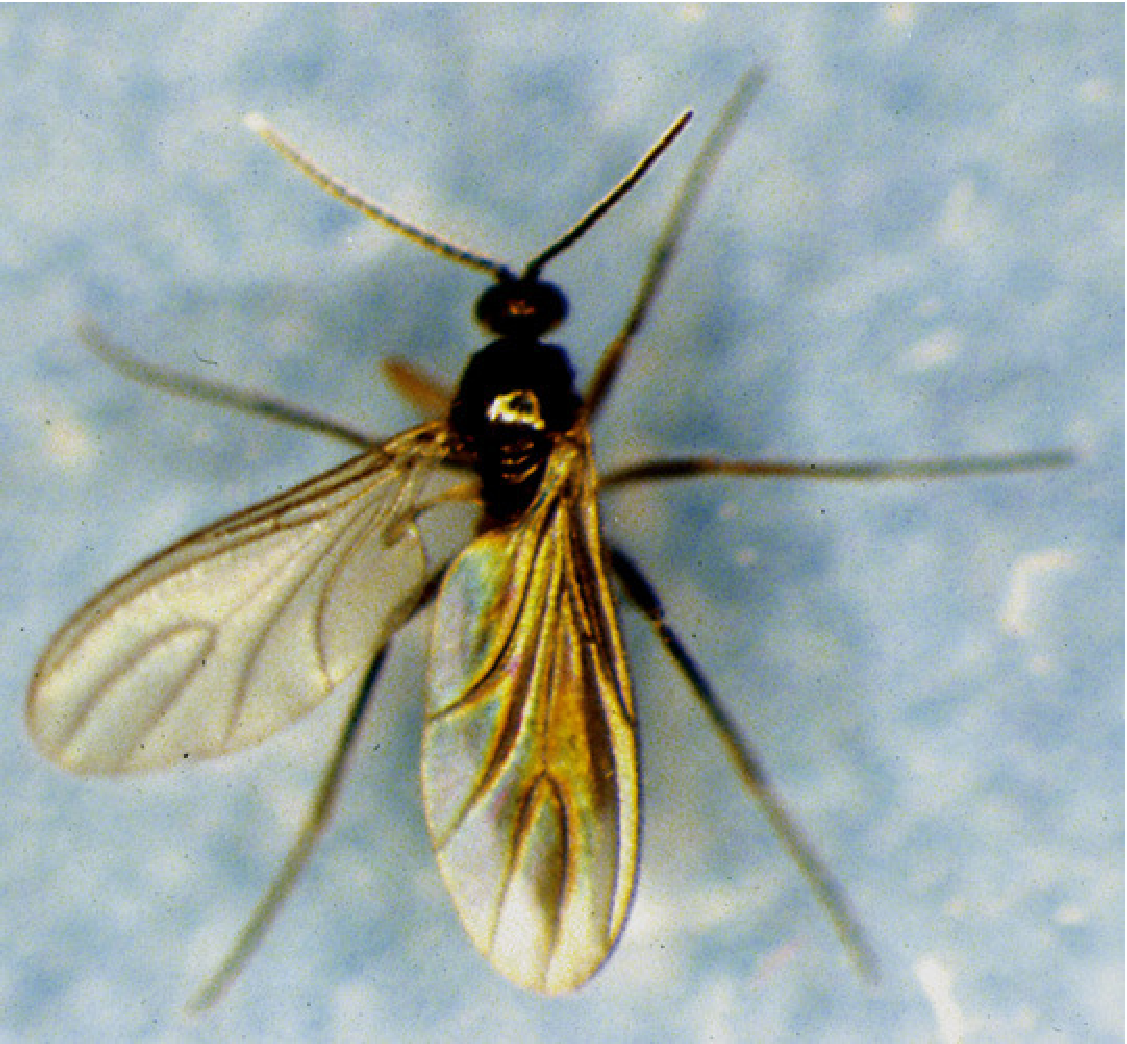
\includegraphics{images/gnat.pdf}}}
%\end{center}
%\caption{Photographs of a gnu (left) and a gnat (right).}
%\label{figure:photos}
%\end{sidewaysfigure}
%
%The results of this comparison are shown in Table~\ref{table:comp1}.
%As can be seen, both volunteers (myself and my advisor) were able to
%correctly classify most of the photographs.  As a result, we gave each
%other little gold stars.
%For those who are interested, Figure~\ref{figure:photos} shows the gnu
%photograph and one of the gnat photographs.
%
%\section{Comparison by Size}
%\index{comparison!size} As can be seen from
%Figure~\ref{figure:photos}, photographs of gnats are slightly larger
%than photographs of gnus.  This leads us to believe that
%statistically, gnats are slightly larger than gnus.  Mathematically,
%we express this as follows:
%\begin{equation}
%S(\mathcal{G}_t) > S(\mathcal{G}_u) \forall
%\mathcal{G}_t,\mathcal{G}_u,
%\end{equation}
%where $\mathcal{G}_t$ is a photograph of a gnat and $\mathcal{G}_u$ is
%a photograph of a gnu.  The $S()$ function calculates the ``size'' of
%the photograph.
%
%\chapter{Conclusions}
%
%Well, there you have it.  My advisor and I were able to tell the
%difference between a photograph of a gnat and a gnu most of the time.
%Also, gnats are larger than gnus, and therefore, they are
%significantly different.
%
%In the future, we plan to apply the techniques developed in this
%research to answer the age old question of whether dogs and ducks are
%the same thing.
%
%\supplementaries
%
%\end{comment}
\bibliography{Thesis_David_Mathews}
%\begin{comment}
%
%\begin{appendices}
%
%\appendix{Appendix A} Well, I really have nothing more to say,
%but wanted to have an appendix.
%
%\end{appendices}
%
%%% Uncomment the following lines if you want to create a glossary
%% \begin{gloss}
%% I don't have a glossary either, but this is what the page would look
%% like if I did.
%% \end{gloss}
%
%
%%% uncomment following lines if you want to create a list of abbreviations
%% \begin{abbreviations}
%% gnu is abbreviated to gnu\\
%% gnat is abbreviated to gnat
%% \end{abbreviations}
%
%%% uncomment next line if you used makeindex to make an index
%%\printindex
%
\begin{vita}

David Michael Mathews was born in Baltimore Maryland on January 12, 2000. After living many years overseas in Papua, Indonesia, David returned to the United States of America to attend South Dakota School of Mines and Technology in the year 2018. During his time at SD Mines, David worked for the electrical engineering department as a student worker, doing such a good job as to even be hired over the summer. In May of 2022, David graduated from the same university with a bachelors in computer engineering. After a summer internship with Raven Industries, David decided to continue his education eventually earning his masters in computer science and engineering in May of 2024. This thesis is David's first scholarly publication.
%  
%Format the vita page according to the following graduate school requirements:
%
%A vita page, not over one page in length, is to be included as the
%last page of all theses and dissertations deposited in the Devereaux
%Library. The vita is to be written in the third person using
%professional style and could contain the following information
%(although you may wish to omit A and B if concerned about identity
%theft):
%\begin{enumerate}[label=\Alph*.]
%\item Place and date of birth.
%
%\item Place and date of high school graduation.
%
%\item Place and date of college graduation—with degree and major.
%
%\item Place and date of receipt of master’s degree—with major.
%
%\item Vocational and professional experience (not summer jobs)—including dates, nature of position, and school or organization.
%
%\item Military experience, with indication of professional relevance—if any.
%
%\item Scholarly publications, exhibits of creative work, membership in professional organizations and honorary societies.
%\end{enumerate}
%  

\end{vita}
%
%
%\end{comment}
\end{document}
